\documentclass[runningheads]{llncs}

\usepackage[T1]{fontenc}
\usepackage[utf8]{inputenc}
\usepackage{amsmath,amssymb,mathtools}
\usepackage{booktabs}
\usepackage{array}
\usepackage{tabularx}
\usepackage{calc}
\usepackage{enumitem}
\usepackage{xcolor}
\usepackage{url}
\usepackage[breaklinks,colorlinks=true, citecolor=blue, linkcolor=magenta]{hyperref}
\usepackage{comment}
\usepackage{float}
\usepackage{listings}
\usepackage{graphicx}
\usepackage{subcaption} 
\usepackage{float}
\usepackage{tikz}
\usetikzlibrary{positioning,arrows.meta,shapes.geometric,matrix,calc}
\usepackage[ruled,      % horizontal rules at top/bottom
            linesnumbered,
            noline,     % no vertical sidebar line
            noend       % no "end" keywords
           ]{algorithm2e}
\usepackage{color,soul}
\allowdisplaybreaks
\usepackage{multirow}
\usepackage{todonotes}
% --- Colors ---
\definecolor{kwblue}{RGB}{0,92,175}
\definecolor{kwgreen}{RGB}{0,120,90}
\definecolor{strred}{RGB}{180,40,40}
\definecolor{numgray}{RGB}{120,120,120}
\definecolor{rulegray}{RGB}{220,220,220}
\definecolor{mGreen}{rgb}{0,0.6,0}
\definecolor{mGray}{rgb}{0.5,0.5,0.5}
\definecolor{mPurple}{rgb}{0.58,0,0.82}
\definecolor{asmBlue}{rgb}{0.1,0.3,0.7}
\definecolor{backgroundMesh}{rgb}{0.97,0.97,0.97}
\definecolor{hlColor}{rgb}{0.98, 0.93, 0.75} 
\definecolor{yhl}{rgb}{0.98, 0.95, 0.75}
\definecolor{rhl}{rgb}{1.0, 0.85, 0.90}
\definecolor{bhl}{rgb}{0.85, 0.90, 1.0}
\newcommand{\highlight}[2]{\colorbox{#1}{#2}}

% --- Listings style ---
\lstdefinestyle{cStyle}{
    language=C,
    basicstyle=\ttfamily\scriptsize,
    columns=fullflexible,
    backgroundcolor=\color{white},
    frame=single,
    rulecolor=\color{rulegray},
    framesep=3pt,
    frameround=tttt,
    keywordstyle=\color{kwblue}\bfseries,
    keywordstyle=[2]\color{kwgreen}\bfseries,
    commentstyle=\color{gray}\itshape,
    stringstyle=\color{strred},
    numbers=left,
    numberstyle=\tiny\color{numgray},
    stepnumber=1,
    numbersep=6pt,
    breaklines=true,
    breakatwhitespace=false,
    keepspaces=true,
    showspaces=false,
    showstringspaces=false,
    showtabs=false,
    tabsize=2,
    xleftmargin=6pt,
    xrightmargin=2pt,
    aboveskip=4pt,
    belowskip=4pt,
    escapeinside={`}{`}
}

\lstdefinestyle{asmStyle}{
    backgroundcolor=\color{white},   
    commentstyle=\color{mGreen}\itshape,
    keywordstyle=\color{asmBlue}\bfseries,
    numberstyle=\tiny\color{mGray},
    basicstyle=\ttfamily\scriptsize,
    breaklines=true,                 
    numbers=left,                    
    numbersep=8pt,                  
    frame=single, % Adds a clean border frame around assembly blocks
    frameround=tttt,
    tabsize=4,
    language=Ant, 
    morekeywords={stmdb, ldrb, cbz, str, bne, lsl, asrs, lsr, movs, bl} 
}

% ---------- TikZ for tree figures ----------
% Node fill colours (flag-tree diagrams)
\definecolor{nodegray}{RGB}{230,228,222}
\definecolor{nodepub}{RGB}{209,239,219}
\definecolor{nodehid}{RGB}{248,215,215}
\definecolor{nodepath}{RGB}{207,231,252}
\definecolor{nodefault}{RGB}{255,236,204}
\definecolor{notegreen}{RGB}{34,139,34}

\tikzset{
  seednode/.style = {circle, minimum size=17pt, inner sep=1pt,
                     fill=nodegray,  draw=gray!60,        thin, font=\scriptsize},
  pubnode/.style  = {circle, minimum size=17pt, inner sep=1pt,
                     fill=nodepub,   draw=green!50!black, thin, font=\scriptsize},
  hidnode/.style  = {circle, minimum size=17pt, inner sep=1pt,
                     fill=nodehid,   draw=red!70!black,   thin, font=\scriptsize},
  pathnode/.style = {circle, minimum size=17pt, inner sep=1pt,
                     fill=nodepath,  draw=blue!60,       thick, font=\scriptsize},
  fltnode/.style  = {circle, minimum size=17pt, inner sep=1pt,
                     fill=nodefault, draw=orange!70,     thick, font=\scriptsize},
  treeedge/.style = {->, >=stealth, thin, gray!60},
  leaflbl/.style  = {font=\tiny, inner sep=0pt}
}


% ---------- Algorithms ----------
\newcommand{\retlabel}[1]{\textcolor{notegreen}{\footnotesize\textit{#1}}}

\newcommand{\algohrule}{\vspace{2pt}\hrule height 0.4pt\vspace{4pt}}
\SetAlgoSkip{medskip}
\SetAlgoInsideSkip{smallskip}
\DontPrintSemicolon
\SetKwComment{Comment}{\quad\textcolor{notegreen}{\(\triangleright\) }}{}
\newcommand{\algocomment}[1]{\Comment*[r]{\textcolor{notegreen}{\footnotesize #1}}}
\newcommand{\outputline}[1]{%
  \noindent\textbf{Return:}\quad #1%
}
\SetKwInOut{Input}{Input}
\SetKwInOut{Output}{Output}
\SetKwFor{ForAll}{for}{do}{}
\SetKwIF{If}{ElseIf}{Else}{if}{}{else if}{else}{}
\SetKwData{Sgn}{Sgn}
 


% ---------- Extra theorem-like environments ----------
\spnewtheorem{assumption}[theorem]{Assumption}{\bfseries}{\itshape}
\spnewtheorem{invariant}[theorem]{Invariant}{\bfseries}{\rmfamily}


% ---------- List spacing ----------
\setlist[itemize]{topsep=2pt,  itemsep=1pt, parsep=0pt}
\setlist[enumerate]{topsep=2pt, itemsep=1pt, parsep=0pt}

% Allow large results figures to be placed at the top/bottom of a text page
\renewcommand{\topfraction}{0.9}
\renewcommand{\bottomfraction}{0.9}
\renewcommand{\textfraction}{0.07}
\renewcommand{\floatpagefraction}{0.75}

% ============================================================
%  macros.tex  --  unified notation for the GGM-tree paper
% ============================================================

% --- Base fields and groups ---------------------------------
\newcommand{\F}{\mathbb{F}}
\newcommand{\C}{\mathbb{C}}
\newcommand{\Fq}{\mathbb{F}_q}
\newcommand{\Mon}{\mathrm{Mon}}
\newcommand{\GL}{\mathrm{GL}}

% --- Security parameter / lengths ---------------------------
\newcommand{\lam}{\lambda}          % security parameter
\newcommand{\seedbytes}{\lambda_s}  % seed length in bytes

% --- Calligraphic sets (abstract model) ---------------------
\newcommand{\calH}{\ensuremath{\mathcal{H}}}
\newcommand{\calR}{\ensuremath{\mathcal{R}}}
\newcommand{\calT}{\ensuremath{\mathcal{T}}}
\newcommand{\calS}{\ensuremath{\mathcal{S}}}
\newcommand{\calF}{\ensuremath{\mathcal{F}}}
\newcommand{\Oracle}{\ensuremath{\mathcal{O}}}

% --- Seeds --------------------------------------------------
\newcommand{\seed}{\ensuremath{\mathsf{seed}}}
\newcommand{\seedsk}{\ensuremath{\mathsf{seed}_{\sk}}}
\newcommand{\seedpk}{\ensuremath{\mathsf{seed}_{\pk}}}
\newcommand{\seedtree}{\ensuremath{\mathsf{seed}_{\mathrm{tree}}}}
\newcommand{\eseed}{\widetilde{s}}  % ephemeral leaf seed  ~s_i

% --- Keys ---------------------------------------------------
\newcommand{\pk}{\ensuremath{\mathsf{pk}}}
\newcommand{\sk}{\ensuremath{\mathsf{sk}}}

% --- Signature components -----------------------------------
\newcommand{\salt}{\ensuremath{\mathsf{salt}}}
\newcommand{\cmt}{\ensuremath{\mathsf{cmt}}}
\newcommand{\msg}{\ensuremath{\mathsf{msg}}}
\newcommand{\rsp}{\ensuremath{\mathsf{rsp}}}
\newcommand{\idx}{\ensuremath{\mathsf{idx}}}
\newcommand{\tpath}{\ensuremath{\mathsf{path}}}  % tree path (avoid clash with tikz \path)

% --- GZKST abstract algorithms ------------------------------
\newcommand{\GZKST}{\ensuremath{\mathsf{GZKST}}}
\newcommand{\Setup}{\ensuremath{\mathsf{Setup}}}
\newcommand{\Expand}{\ensuremath{\mathsf{Expand}}}
\newcommand{\Chal}{\ensuremath{\mathsf{Chal}}}
\newcommand{\Decide}{\ensuremath{\mathsf{Decide}}}
\newcommand{\Publish}{\ensuremath{\mathsf{Publish}}}
\newcommand{\Recon}{\ensuremath{\mathsf{Recon}}}
\newcommand{\sig}{\ensuremath{\mathsf{sig}}}
\newcommand{\resp}{\ensuremath{\mathsf{resp}}}
\newcommand{\Extract}{\ensuremath{\mathsf{Extract}}}

% --- LESS-specific algorithms -------------------------------
\newcommand{\CF}{\ensuremath{\mathsf{CF}}}
\newcommand{\Blind}{\ensuremath{\mathsf{Blind}}}
\newcommand{\CosetRep}{\ensuremath{\mathsf{CosetRep}}}
\newcommand{\RREF}{\ensuremath{\mathsf{RREF}}}
\newcommand{\BuildGGM}{\ensuremath{\mathsf{BuildGGM}}}
\newcommand{\GGMPath}{\ensuremath{\mathsf{GGMPath}}}
\newcommand{\RebuildGGM}{\ensuremath{\mathsf{RebuildGGM}}}
\newcommand{\LabelLeaves}{\ensuremath{\mathsf{LabelLeaves}}}
\newcommand{\ComputeSeeds}{\ensuremath{\mathsf{ComputeSeeds}}}
\newcommand{\SampleChallenge}{\ensuremath{\mathsf{SampleChallenge}}}
\newcommand{\SampleGenerator}{\ensuremath{\mathsf{SampleGenerator}}}
\newcommand{\SampleMonomial}{\ensuremath{\mathsf{SampleMonomial}}}
\newcommand{\SeedLeaves}{\ensuremath{\mathsf{SeedLeaves}}}
\newcommand{\CheckCosetRep}{\ensuremath{\mathsf{CheckCosetRep}}}

% --- MEDS/CROSS-specific ------------------------------------
\newcommand{\SeedTree}{\ensuremath{\mathsf{SeedTree}}}
\newcommand{\SeedTreePath}{\ensuremath{\mathsf{SeedTreePath}}}
\newcommand{\BuildSeeds}{\ensuremath{\mathsf{BuildSeeds}}}
\newcommand{\ReconstructSeeds}{\ensuremath{\mathsf{ReconstructSeeds}}}
\newcommand{\pimap}[2]{\pi_{#1,#2}}

% --- Cryptographic primitives -------------------------------
\newcommand{\GGM}{\ensuremath{\mathsf{GGM}}}
\newcommand{\Hash}{\ensuremath{\mathsf{Hash}}}
\newcommand{\XOF}{\ensuremath{\mathsf{XOF}}}
\newcommand{\SHAKE}{\ensuremath{\mathsf{SHAKE}}}
\newcommand{\PRG}{\ensuremath{\mathsf{G}}}               % PRG symbol: G:{0,1}^lambda -> {0,1}^{2lambda}
\newcommand{\PRGl}{\ensuremath{\mathsf{G_0}}}            % left half of PRG output
\newcommand{\PRGr}{\ensuremath{\mathsf{G_1}}}            % right half of PRG output

% --- Signature scheme algorithms ----------------------------
\newcommand{\KeyGen}{\ensuremath{\mathsf{KeyGen}}}
\newcommand{\Sign}{\ensuremath{\mathsf{Sign}}}
\newcommand{\Verify}{\ensuremath{\mathsf{Verify}}}
% --- Flag array (implementation level) ----------------------
\newcommand{\flags}{\mathtt{flags}}  % the flag array in algorithms

% --- Misc operators -----------------------------------------
\DeclareMathOperator{\supp}{supp}
\newcommand{\getsr}{\mathrel{\xleftarrow{\$}}}  % sample uniformly

% ============================================================
% Unicode compatibility for pdflatex
% ============================================================
\DeclareUnicodeCharacter{03BB}{\ensuremath{\lambda}}
\DeclareUnicodeCharacter{03A0}{\ensuremath{\Pi}}
\DeclareUnicodeCharacter{03A3}{\ensuremath{\Sigma}}
\DeclareUnicodeCharacter{2113}{\ensuremath{\ell}}
\DeclareUnicodeCharacter{2190}{\ensuremath{\leftarrow}}
\DeclareUnicodeCharacter{00B7}{\ensuremath{\cdot}}
\DeclareUnicodeCharacter{03C0}{\ensuremath{\pi}}
\DeclareUnicodeCharacter{03C4}{\ensuremath{\tau}}
\DeclareUnicodeCharacter{1D4AE}{\ensuremath{\mathcal{S}}}
\DeclareUnicodeCharacter{2192}{\ensuremath{\to}}
\DeclareUnicodeCharacter{21D0}{\ensuremath{\Leftarrow}}
\DeclareUnicodeCharacter{2260}{\ensuremath{\neq}}
\DeclareUnicodeCharacter{2265}{\ensuremath{\geq}}
\DeclareUnicodeCharacter{2264}{\ensuremath{\leq}}
\DeclareUnicodeCharacter{2212}{\ensuremath{-}}
\DeclareUnicodeCharacter{2208}{\ensuremath{\in}}
\DeclareUnicodeCharacter{2209}{\ensuremath{\notin}}
\DeclareUnicodeCharacter{2218}{\ensuremath{\circ}}
\DeclareUnicodeCharacter{2227}{\ensuremath{\wedge}}
\DeclareUnicodeCharacter{2200}{\ensuremath{\forall}}
\DeclareUnicodeCharacter{2308}{\ensuremath{\lceil}}
\DeclareUnicodeCharacter{2309}{\ensuremath{\rceil}}
\DeclareUnicodeCharacter{00D7}{\ensuremath{\times}}
\DeclareUnicodeCharacter{2013}{--}
\DeclareUnicodeCharacter{2014}{---}
\DeclareUnicodeCharacter{2019}{'}

% Pandoc list compatibility (kept for safety, but no longer generated)
\providecommand{\tightlist}{}
\newcommand{\SF}{\ensuremath{\mathsf{SF}}}
\newcommand{\ParseHash}{\ensuremath{\mathsf{ParseHash}}}
\newcommand{\SeedPath}{\ensuremath{\mathsf{SeedTreeToPath}}}
\newcommand{\PathToSeedTree}{\ensuremath{\mathsf{PathToSeedTree}}}
\newcommand{\ExpandInvMat}{\ensuremath{\mathsf{ExpandInvMat}}}
\newcommand{\ExpandSys}{\ensuremath{\mathsf{ExpandSystMat}}}
\newcommand{\DecompressG}{\ensuremath{\mathsf{DecompressG}}}
\newcommand{\CompressG}{\ensuremath{\mathsf{CompressG}}}
\newcommand{\Compress}{\ensuremath{\mathsf{Compress}}}
\newcommand{\ExpandSystMat}{\ensuremath{\mathsf{ExpandSystMat}}}
\newcommand{\ExpandFqs}{\ensuremath{\mathsf{ExpandFqs}}}
\newcommand{\Solve}{\ensuremath{\mathsf{Solve}}}
\newcommand{\ToBytes}{\ensuremath{\mathsf{ToBytes}}}
\newcommand{\SeedTreeToPath}{\ensuremath{\mathsf{SeedTreeToPath}}}


%% ── Keyword styling (mimic handwriting informality) ──────────
\SetKwFor{ForAll}{for}{do}{}
\SetKwIF{If}{ElseIf}{Else}{if}{}{else if}{else}{}
\SetKwData{pk}{\ensuremath{\mathsf{pk}}}
\SetKwData{sk}{\ensuremath{\mathsf{sk}}}
\SetKwData{Sgn}{\ensuremath{\mathsf{Sgn}}}

% --- Added in restructure: generic round functions -----------
\newcommand{\Commit}{\ensuremath{\mathsf{Commit}}}
\newcommand{\Resp}{\ensuremath{\mathsf{Resp}}}
\newcommand{\ChkRnd}{\ensuremath{\mathsf{Check}}}
\newcommand{\Sig}{\ensuremath{\Sigma}}
\newcommand{\vect}{\ensuremath{\mathrm{vec}}}
\newcommand{\Mat}{\ensuremath{\mathcal{C}}}
\newcommand{\Matd}{\ensuremath{\mathcal{D}}}

% --- Revision marking ----------------------------------------
% New or changed text is wrapped in \chg{...} and shown in blue.
% For the final version, replace the definition below by
%   \newcommand{\chg}[1]{#1}
\DeclareRobustCommand{\chg}[1]{#1}
% Blue highlights mark passages newly written or revised in the October 25 edit.
% For a clean final version, change \showrevisionstrue to \showrevisionsfalse.
% The pre-existing \chg commands are intentionally independent of this switch.
\newif\ifshowrevisions
\showrevisionstrue
\definecolor{revisionblue}{RGB}{0,72,185}
\ifshowrevisions
  \DeclareRobustCommand{\rev}[1]{{\color{revisionblue}#1}}
  \DeclareRobustCommand{\revon}{\color{revisionblue}}
  \DeclareRobustCommand{\revoff}{\color{black}}
\else
  \DeclareRobustCommand{\rev}[1]{#1}
  \DeclareRobustCommand{\revon}{}
  \DeclareRobustCommand{\revoff}{}
\fi
% Placeholder for a value the authors must fill in from a cited source.
\providecommand{\PH}{{\color{red}\textbf{??}}}

\usepackage{lineno}
\setcounter{tocdepth}{1} % Table of contents for llncs
\renewcommand{\linenumberfont}{\normalfont\small\color{red}}%
%\linenumbers

% CASCADE submissions are anonymous. Set \anonymoustrue to blind the paper.
\newif\ifanonymous
\anonymoustrue   % CASCADE is blind-refereed; set \anonymousfalse for camera-ready

\begin{document}

\title{So Long, and Thanks for All the Seeds: Attacking GGM-trees in Post-quantum signatures}
\titlerunning{So Long, and Thanks for All the Seeds}


\ifanonymous
\author{}
\authorrunning{}
\institute{}
\else
\author{Gustavo Banegas\inst{1} \and Damya Bouizegarene\inst{2}}
\authorrunning{Banegas and Bouizegarene}
\institute{Inria, LIX, CNRS, École Polytechnique,
Institut Polytechnique de Paris\\
  Palaiseau, France\\
  \email{gustavo@cryptme.in}\\
  \and
  T\'el\'ecom Paris,
  Palaiseau, France\\
  \email{bouizegarene.damya@gmail.com}\\
}
\fi

\maketitle

\begin{abstract}
Post-quantum signatures based on Fiat--Shamir-transformed 
zero-knowledge protocols use GGM seed trees to compress 
ephemeral randomness. Faults in seed publication can reveal 
hidden seeds and enable secret-key recovery.
We introduce the Generic ZK Seed Tree (GZKST), 
formalise its correctness and seed-hiding invariants, 
and classify existing fault attacks across six components. 
This taxonomy guides us to a new fault surface in the MEDS 
reference implementation. We derive generic key-recovery 
bounds and show that, under independent uniform challenge 
indices, one effective faulted signature recovers the full 
MEDS key with probability at least $0.987$ for every 
parameter set, with fewer than $1.02$ effective faults 
expected. Finally, we demonstrate three function-level 
clock-glitch attacks against the MEDS seed-path routine 
on an ARM Cortex-M4, enabling root-seed disclosure, 
subtree recovery, or individual hidden-leaf leakage. 
We also evaluate countermeasures and discuss the limitations 
of verify-before-release when path construction and 
reconstruction share code.
\keywords{GGM tree \and Zero-knowledge signatures \and Fault attacks \and
Post-quantum cryptography \and Seed compression}
\end{abstract}
  \ifanonymous\else
  \makeatletter%
\begingroup%
 \makeatletter%
 \def\@thefnmark{$*$}\relax%
 \@footnotetext{\relax%
   Author list in alphabetical order; see \url{https://ams.org/profession/leaders/CultureStatement04.pdf}.
   This work was supported by the HYPERFORM consortium, funded by France through Bpifrance, and by the France
   2030 program under grant agreement ANR-22-PETQ-0008 PQ-TLS.
\def\ymdtoday{\leavevmode\hbox{\the\year-\twodigits\month-\twodigits\day}}\def\twodigits#1{\ifnum#1<10 0\fi\the#1}%
  Date of this document: \ymdtoday.%
 }%
\endgroup
\fi

\section{Introduction}
\label{sec:intro}
Digital signatures underpin firmware updates, secure boot, messaging and
public-key infrastructures, and the schemes deployed today rest on integer
factorisation or on the Elliptic Curve Discrete Logarithm Problem, both of
which a large quantum computer would solve with Shor's algorithm. Among the
most promising replacements are signatures obtained by applying the
Fiat--Shamir transform~\cite{DagdelenFG13,FiatS86} to a zero-knowledge
identification protocol repeated in parallel --- LESS~\cite{LESS-spec},
CROSS~\cite{CROSSspec} and MEDS~\cite{ChouNPRRST23,MEDS_PQC} among them. Their
weak point is signature size, and the standard remedy is
\GGM-tree seed compression: the $t$ ephemeral secrets are derived from a single
root seed, so that the signer publishes a handful of internal nodes rather than
$t$ independent seeds.

During signing, only the seeds of the revealed rounds may be released; the
challenge-dependent ones must stay hidden. This is the single point at which
zero knowledge is enforced in the implementation, and recent work has shown it
to be a fault-attack surface: a fault in the seed-publication logic can leak a
hidden seed alongside the zero-knowledge response of the same round, which is
enough for key recovery or universal
forgery~\cite{FaultToForge2025,ZKFault}.


%In 2022, the National Institute 
%of Standards and Technology selected the first set of post-quantum 
%digital signature schemes as part of its standardization process, 
%marking a major step toward the deployment of quantum-resistant 
%cryptography.





\paragraph{Why seed trees, and not one scheme.}
The three schemes named above have all now left the NIST additional-signatures
process: MEDS was not selected for the second round, and CROSS and LESS were
eliminated at the end of it~\cite{NISTIR8610}. It would be a mistake to read
this as closing the subject. The compression technique is not specific to
those designs: it is the standard way to shrink any Fiat--Shamir signature
built from a parallel-repeated identification protocol, and FAEST, SDitH and
MQOM --- all of which did advance --- publish an all-but-one vector commitment
derived from the same tree. What we analyse is the mechanism, not its host. We
attack MEDS because its reference implementation realises that mechanism in
its cleanest form, and the conclusions transfer to any scheme publishing a
seed-tree path. The timing is favourable rather than late: the third round is
explicitly an implementation-security phase.

\subsection{Related Work}
\label{sec:relwork}
Fault attacks on seed-tree-based post-quantum signatures are an active line of
work. ZKFault~\cite{ZKFault} faults the seed publication of LESS-v1, extended
to CROSS, disclosing hidden ephemeral seeds and recovering secret material.
Fault-to-Forge~\cite{FaultToForge2025} revisits LESS-v2, whose incomplete tree
defeats that strategy, and finds new injection points in tree generation and
seed publication, showing that secret-equivalent information already suffices
for universal forgery. The attack of~\cite{HuangHHYSTY26} avoids the tree
altogether, using iteration-skip and loop-abort faults in the
digest-preprocessing step that precedes tree generation. Elsewhere in the
family,~\cite{cryptoeprint:2026/1266} faults tree generation in
PERK~\cite{BettaiebBDEGKP24},~\cite{JendralD25} targets FAEST,
and~\cite{BandaBK26} targets Mirath and RYDE.

We unify these results under a single Generic ZK Seed Tree abstraction,
formalising the invariants they implicitly exploit, and add practical fault
attacks against MEDS.

\paragraph{Our Contributions.}
This work provides a unified analysis of fault attacks against
post-quantum signature schemes relying on seed-tree compression.
Our main contributions are as follows:
\begin{itemize}

\item \textbf{Generic Seed-Tree Abstraction.}
We introduce the \emph{Generic ZK Seed Tree} (GZKST), a unified model
capturing the seed-tree generation mechanisms used in schemes such as
LESS-v2, MEDS, and CROSS.

\item \textbf{Unified View of Existing Attacks.}
We show that previously proposed fault attacks against LESS-v1 and
LESS-v2 can be interpreted as violations of a common seed-hiding
invariant.

\item \textbf{A Taxonomy of Fault Surfaces.}
We classify every published fault attack on this family by which component
of the abstraction it corrupts (Section~\ref{sec:taxonomy}), showing that
five independent attacks against four schemes occupy only three of six
components. The empty cells are predictions, and one of them led us
directly to a new attack surface in the MEDS reference implementation
that has no analogue in prior work.

\item \textbf{Query Complexity Analysis.}
We derive bounds on the number of faulted signatures required for
secret-key recovery and show that only a small number of successful
queries is needed for all MEDS parameter sets.

\item \textbf{Practical Attacks on MEDS.}
We show fault attacks against the MEDS reference
implementation on an ARM Cortex-M4 using a ChipWhisperer-Lite,
revealing several fault surfaces that enable complete or partial
seed-tree disclosure.

\item \textbf{Countermeasures for MEDS, and their limits.}
We propose and evaluate three families of countermeasures. We also show
that the obvious defence --- verifying a signature before releasing it ---
is weaker than it looks against this particular implementation, because
path construction and path reconstruction share a single function, so the
same glitch at the same code offset defeats both passes
(Section~\ref{sec:counter}).

\end{itemize}



\section{Background}
\label{sec:background}
% ============================================================
%  Section 2 – Background
% ============================================================
\subsection{GGM trees}
The Goldreich--Goldwasser--Micali construction~\cite{GGM86} builds a
pseudorandom function from a pseudorandom generator by iterated expansion along
the branches of a binary tree indexed by the input bits. It is the construction
studied throughout this work.


\begin{definition}[GGM Tree]
\label{def:ggm}
Let $\PRG : \{0,1\}^{\lam} \to \{0,1\}^{2\lam}$ be a length-doubling pseudorandom
generator, decomposed as $\PRG(x) = (\PRGl(x),\, \PRGr(x))$, where $\PRGl$ and
$\PRGr$ each output $\lam$ bits.  Given a root seed
$\seed_r \in \{0,1\}^{\lam}$ and a depth $d$, the \emph{GGM tree} is a complete
binary tree of depth $d$ in which:
\begin{itemize}
  \item the root holds $\seed_r$;
  \item each internal node $v$ storing seed $s$ generates its left child as
        $\PRGl(s)$ and its right child as $\PRGr(s)$;
  \item the $2^{d}$ leaves are the \PRG\ outputs at depth $d$.
\end{itemize}
\end{definition}

\revon
For a secure PRG, the seed of a punctured leaf remains computationally
hidden even when the legitimate seeds of other leaves are disclosed.
Structurally, a published ancestor permits forward derivation of every leaf
in its subtree. These computational and structural statements are distinct
(see Figure~\ref{fig:less-trees}).
\revoff

\paragraph{Incomplete \GGM\ trees.}
When the number of required leaves $t$ is not a power of $2$, a scheme may use an
\emph{incomplete} tree: leaves appear at multiple levels, and internal nodes near
the bottom may have fewer than two children or act as leaves themselves. This
reduces memory and computation, but the additional index-tracking logic introduces
new fault surfaces. The scheme may also use the first $t$ leaves of the tree.
%as detailed in Section~\ref{sec:theoretical}.

% ============================================================
\paragraph{The common template.}
\label{sec:template}
% ============================================================

All schemes considered here share one skeleton, worth stating once. A $3$- or
$5$-pass identification protocol is repeated $t$ times in parallel and made
non-interactive by Fiat--Shamir. Round $i$ needs a fresh ephemeral secret,
derived from a leaf seed $\eseed_i$; the $t$ leaf seeds are the leaves of one
\GGM\ tree, so the signer stores $\lambda$ bits instead of $t\lambda$.

The challenge $\mathbf{c}$ has fixed weight $w$ and splits the rounds in two.
For the $w$ \emph{hidden} rounds ($i \in \calH$) the signer publishes a
response $\resp_i$ combining the ephemeral secret with the long-term key, so
$\eseed_i$ must stay secret: $\resp_i$ and $\eseed_i$ together determine that
key. For the $t-w$ \emph{revealed} rounds ($i \in \calR$) the seed itself is
released and the verifier recomputes the commitment.

Releasing $t-w$ individual seeds would undo the compression, so the signer
publishes instead the boundary of the hidden subtree --- a small set of
internal nodes from which exactly the revealed leaves, and no others, can be
recomputed. We call this set the \emph{path}. Computing it is the only place
in signing where the code decides, per node, whether a seed may be released,
and that decision is the object of this paper: \chg{it is what the attacks
of~\cite{ZKFault,FaultToForge2025}, and every attack we mount in
Section~\ref{sec:app}, corrupt. The remaining attacks surveyed in
Section~\ref{sec:relwork} reach the same leak through other components;
Section~\ref{sec:taxonomy} places them.}

% ============================================================
\subsection{The MEDS signature scheme}
\label{sec:meds}
% ============================================================

The Matrix Equivalence Digital Signature (MEDS) scheme~\cite{ChouNPRRST23} is
a code-based signature whose security rests on the hardness of the Matrix Code
Equivalence (MCE) problem. Because the practical attacks of
Section~\ref{sec:app} target the MEDS reference implementation, we describe it
in more detail than the other instances.

\paragraph{Matrix codes and the MCE problem.}
A \emph{matrix code} of dimension $k$ is a $k$-dimensional $\Fq$-subspace
$\Mat \subseteq \Fq^{m \times n}$. Two matrix codes $\Mat, \Matd$ are
\emph{equivalent} if there exist $A \in \GL_m(q)$ and $B \in \GL_n(q)$ with
\[
  \Matd \;=\; A\,\Mat\,B \;:=\; \{\, A\,C\,B \;:\; C \in \Mat \,\}.
\]

\begin{definition}[Matrix Code Equivalence]
\label{def:mce}
Given two $k$-dimensional matrix codes $\Mat, \Matd \subseteq \Fq^{m\times n}$,
the \emph{MCE problem} asks for a pair $(A,B) \in \GL_m(q) \times \GL_n(q)$
such that $\Matd = A\,\Mat\,B$.
\end{definition}

In implementations a matrix code is handled through a generator matrix
$G \in \Fq^{k \times mn}$ whose $k$ rows are the vectorisations
$\vect(C_1),\ldots,\vect(C_k)$ of a basis of $\Mat$. Write $\pimap{A}{B}$ for
the induced row-wise map
\[
  \pimap{A}{B}\bigl(\vect(C)\bigr) \;=\; \vect\bigl(A\,C\,B\bigr),
\]
extended to generator matrices by applying it to each row. Since a generator
matrix fixes a basis but equivalence only relates the underlying
\emph{subspaces}, the relation between two generator matrices of equivalent
codes carries a third, unknown ingredient: a change of basis
$T \in \GL_k(q)$. Concretely, $G_0$ and $G_1$ generate equivalent codes if and
only if there exists a triple $(A,B,T)$ with
\begin{equation}
  \label{eq:mce-gen}
  G_1 \;=\; T \cdot \pimap{A}{B}(G_0),
  \qquad\text{equivalently}\qquad
  G_1 \;=\; \SF\bigl(\pimap{A}{B}(G_0)\bigr),
\end{equation}
where $\SF$ denotes the systematic form, which absorbs $T$ by fixing a
canonical basis.

\revon
\chg{The unknown basis change $T$ is central to the hardness: with $T$ fixed the
\revoff
relations are linear in $(A,B^{-1})$, which MEDS key generation exploits to
sample keys, whereas with $T$ unknown \eqref{eq:mce-gen} is a system of
bilinear equations (Remark~\ref{rem:mce-hardness} in
Appendix~\ref{app:algs}). MCE is Tensor-Isomorphism-complete~\cite{GrochowQiao23};
see~\cite{ReijndersST23,NarayananQT24} for the best known classical
algorithms. Subroutine names follow the reference
specification~\cite{ChouNPRRST23,MEDS_PQC} and are summarised in
Table~\ref{tab:meds-notation} (Appendix~\ref{app:algs}).}

\paragraph{Key generation.}
Key generation (Algorithm~\ref{alg:keygen_meds}, Appendix~\ref{app:algs})
expands a public seed into $G_0$ and then produces $s-1$ equivalent codes: for
each $i$ it samples $T_i \in \GL_k(q)$, recovers $(A_i,B_i^{-1})$ from
$T_i G_0$ by the linear solve of Remark~\ref{rem:mce-hardness}, and publishes
$G_i \leftarrow \SF(\pimap{A_i}{B_i}(G_0))$. The secret key retains the pairs
\revon
$(A_i^{-1},B_i^{-1})$; these pairs are sufficient to construct signing-equivalent secret information.
\revoff

\paragraph{Signing and the role of the seed tree.}
Algorithm~\ref{alg:sign_meds} follows the template just described. A fresh $\delta$ is expanded into a root seed
$\rho$ and a salt $\alpha$; \chg{line~\ref{alg:meds:tree}} grows the \GGM\ tree of
Definition~\ref{def:ggm} from $\rho$, yielding the $t$ ephemeral leaf seeds
$\sigma_0,\ldots,\sigma_{t-1}$. Each $\sigma_i$ is expanded into an ephemeral
equivalence $(\tilde{A}_i, \tilde{B}_i)$, and round $i$ commits to the
resulting generator matrix
$\tilde{G}_i = \SF(\pimap{\tilde{A}_i}{\tilde{B}_i}(G_0))$ by hashing its
non-systematic part. Hashing all $t$ commitments together with the message
gives the digest $d$, parsed into the weight-$w$ challenge
$\mathbf{h} = (h_0,\ldots,h_{t-1})$.

For each hidden round ($h_i > 0$) the signer publishes the response pair
\begin{equation}
  \label{eq:meds-resp}
  (\mu_i, \nu_i) \;=\; \bigl(\tilde{A}_i A_{h_i}^{-1},\;
                             B_{h_i}^{-1} \tilde{B}_i\bigr),
\end{equation}
and for the revealed rounds the seeds are released compactly through the path
$p \leftarrow \SeedTreeToPath_t(\mathbf{h},\rho,\alpha)$ computed at
\chg{line~\ref{alg:meds:path}},
the target of every attack in Section~\ref{sec:app}.

\begin{algorithm}[tb]
\footnotesize
\setlength{\algomargin}{0.9em}
\caption{MEDS signing (simplified).}
\label{alg:sign_meds}
\KwIn{Secret key $\sk$, message $m$}
\KwOut{Signed message $m_s$}

Parse $\sk$ to recover $\sigma_{G_0}$, $A_i^{-1}$, $B_i^{-1}$, $i=1,\ldots,s-1$;\quad
$G_0 \leftarrow \ExpandSystMat(\sigma_{G_0})$\;
$\delta \xleftarrow{\$} \mathcal{B}^{\ell_{\mathrm{sec\_seed}}}$;\quad
$\rho,\, \alpha \leftarrow \XOF(\delta,\, \ell_{\mathrm{tree\_seed}},\, \ell_{\mathrm{salt}})$\;
$(\sigma_0, \ldots, \sigma_{t-1}) \leftarrow \SeedTree_t(\rho,\, \alpha)$\label{alg:meds:tree}
\tcp*[r]{\GGM\ tree, Def.~\ref{def:ggm}}

\For{$i = 0$ \KwTo $t-1$}{
    $\sigma'_i \leftarrow \bigl(\alpha \mid \sigma_i \mid \ToBytes(2^{1+\lceil\log_2 t\rceil}+i,4)\bigr)$;\quad
    $\sigma_{\tilde{A}_i},\, \sigma_{\tilde{B}_i} \leftarrow \XOF(\sigma'_i,\, \ell_{\mathrm{pub\_seed}},\, \ell_{\mathrm{pub\_seed}})$\;
    $\tilde{A}_i \leftarrow \ExpandInvMat(\sigma_{\tilde{A}_i}, m)$;\quad
    $\tilde{B}_i \leftarrow \ExpandInvMat(\sigma_{\tilde{B}_i}, n)$;\quad
    $\tilde{G}_i \leftarrow \SF\!\bigl(\pimap{\tilde{A}_i}{\tilde{B}_i}(G_0)\bigr)$
    \tcp*[r]{$\perp\Rightarrow$ resample}
}

$d \leftarrow H\!\bigl(\Compress(\tilde{G}_0[;k,mn{-}1]) \mid \cdots \mid \Compress(\tilde{G}_{t-1}[;k,mn{-}1]) \mid m\bigr)$\;
$(h_0,\ldots,h_{t-1}) \leftarrow \ParseHash_{s,t,w}(d)$
\tcp*[r]{weight-$w$ challenge}

\For{$i = 0$ \KwTo $t-1$ \textbf{with} $h_i > 0$}{
    $\mu_i \leftarrow \tilde{A}_i A_{h_i}^{-1}$;\quad
    $\nu_i \leftarrow B_{h_i}^{-1} \tilde{B}_i$;\quad
    append $\bigl(\Compress(\mu_i) \mid \Compress(\nu_i)\bigr)$ to $v$\;
}

$p \leftarrow \SeedTreeToPath_t(h_0,\ldots,h_{t-1},\rho,\alpha)$\label{alg:meds:path}
\tcp*[r]{\textbf{attack target}}
\Return $m_s \leftarrow \bigl(v \mid p \mid d \mid \alpha \mid m\bigr)$
\end{algorithm}

\paragraph{Verification.}
Verification (Algorithm~\ref{alg:verify_meds}, Appendix~\ref{app:algs})
recomputes the challenge from $d$, runs $\PathToSeedTree_t$ to recover the
$t-w$ revealed seeds, rebuilds every $\hat{G}_i$---from $(\mu_i,\nu_i)$ and
$G_{h_i}$ when $h_i > 0$, from the recovered seed when $h_i = 0$---and accepts
iff the recomputed digest equals $d$. Note that for hidden rounds the verifier
never uses $\sigma_i$: the seed of a hidden round is simply absent from an
honest signature.

\paragraph{Secret-extraction opportunity.}
This last observation is what the attacks exploit. Fix a hidden round $i$ with
$h_i = j$. The signature already contains $(\mu_i,\nu_i)$
from~\eqref{eq:meds-resp}. If an attacker additionally obtains $\sigma_i$, it
expands it into $(\tilde{A}_i,\tilde{B}_i)$ and reads off
\begin{equation}
  \label{eq:meds-extract}
  A_j^{-1} \;=\; \tilde{A}_i^{-1} \mu_i,
  \qquad
  B_j^{-1} \;=\; \nu_i \tilde{B}_i^{-1},
\end{equation}
\revon
by two matrix inversions and two multiplications over $\Fq$. Correct seed publication prevents this pair of revelations during
an honest signing execution.
\revoff

\begin{table}[htbp]
\centering
\caption{MEDS parameter sets~\cite{ChouNPRRST23}; MEDS uses $n{=}m{=}k$. \chg{For
an effective root fault, the last three columns give
$p_{\min} = 1-((s-2)/(s-1))^{w}$ of Proposition~\ref{prop:alg-correctness},
\revon
the probability $\Pr[Q{=}1]$ that one \emph{effective root disclosure}
covers every long-term matrix pair, and the exact expected number $\mathbb{E}[Q]$ of effective faulted
\revoff
signatures needed (Appendix~\ref{app:proof-query}).}}
\label{tab:scheme-params}
\setlength{\tabcolsep}{4pt}
\small
\begin{tabular}{@{}lrrrcl rrr@{}}
\toprule
\textbf{Parameter set} & $t$ & $w$ & $s$ & \chg{\textbf{Level}} & \textbf{Field}
 & $p_{\min}$ & \chg{$\Pr[Q{=}1]$} & \chg{$\mathbb{E}[Q]$} \\
\midrule
MEDS-9923   & 1152 & 14 & 4 & I   & $n{=}14,\,q{=}4093$ & 0.9966 & \chg{0.9897} & \chg{1.0103} \\
MEDS-13220  &  192 & 20 & 5 & I   & $n{=}14,\,q{=}4093$ & 0.9968 & \chg{0.9873} & \chg{1.0127} \\
MEDS-41711  &  608 & 26 & 4 & III & $n{=}22,\,q{=}4093$ & 1.0000 & \chg{0.9999} & \chg{1.0001} \\
MEDS-69497  &  160 & 36 & 5 & III & $n{=}22,\,q{=}4093$ & 1.0000 & \chg{0.9999} & \chg{1.0001} \\
MEDS-134180 &  192 & 52 & 5 & V   & $n{=}30,\,q{=}2039$ & 1.0000 & \chg{1.0000} & \chg{1.0000} \\
MEDS-167717 &  112 & 66 & 6 & V   & $n{=}30,\,q{=}2039$ & 1.0000 & \chg{1.0000} & \chg{1.0000} \\
\bottomrule
\end{tabular}
\end{table}

% ============================================================
\subsection{Other instances: LESS-v2, CROSS, and MPCitH}
\label{sec:others}
% ============================================================

The other schemes differ in the algebra but not in the mechanism, and we
record only what the fault analysis needs.

\textbf{LESS-v2}~\cite{LESS-spec} applies Fiat--Shamir to a $3$-pass sigma
protocol over the Canonical Form Linear Equivalence problem. Its long-term
secret is a set of monomial matrices $\pi_1,\ldots,\pi_{s-1} \in \Mon_n(q)$,
and a hidden round publishes the coset representative
$\CosetRep(\pi_{b[i]} \circ \tilde{\pi}^*_i)$. Two structural differences from
MEDS matter, because the attacks of~\cite{ZKFault,FaultToForge2025} turn on
them: the tree is \emph{incomplete}, so leaves sit at two depths and the
implementation carries \chg{per-level leaf-offset arrays} to locate them; and the
path is computed from an explicit auxiliary \emph{flag tree}, with
$\LabelLeaves$ writing $\calF(\mathrm{leaf}_i) = \mathbf{1}[i \in \calH]$ and
$\ComputeSeeds$ propagating $\calF(v) = \calF(\ell) \vee \calF(r)$ upwards.
Both the \chg{leaf-offset arrays} and the flag array are state that MEDS does not
have, and hence fault surface that MEDS does not have\chg{; MEDS has a different
piece of state instead, a cursor into the sorted list of hidden leaves
(Section~\ref{sec:app})}. Recovering $\pi_{b[i]}$
from the response together with $\eseed_i$ is the column-extraction argument
of Lemma~1 in~\cite{FaultToForge2025}, structurally the analogue
of~\eqref{eq:meds-extract}.

\textbf{CROSS}~\cite{CROSSspec} builds on the Restricted Syndrome Decoding
Problem~\cite{BaldiBPSWW24} through a $5$-pass protocol. Its second challenge
is a binary weight-$w$ vector, so $\calH$ and $\calR$ have exactly the shape
they have in MEDS. Each leaf seed expands into $(\mathbf{e}'_i,
\mathbf{u}'_i)$, and a hidden round publishes $\mathbf{v}_i = \mathbf{e} \star
(\mathbf{e}'_i)^{-1}$, where $\mathbf{e}$ is the long-term R-SDP solution; an
attacker holding $\mathbf{v}_i$ and $\eseed_i$ recovers $\mathbf{e} =
\mathbf{v}_i \star \mathbf{e}'_i$ directly, which is how
ZKFault~\cite{ZKFault} achieves key recovery from one fault. CROSS also
authenticates the $w$ commitments the verifier cannot recompute with a Merkle
tree; this is orthogonal to seed hiding.

\textbf{MPCitH and VOLEitH schemes} use the tree in a superficially different
but structurally identical way. For each of $\tau$ repetitions the challenge
selects one hidden party index, and the signer publishes the \emph{co-path} of
siblings from that leaf to the root, letting the verifier recompute the other
$N-1$ shares. Mirath and RYDE use a forest of $\tau$ trees; FAEST and SDitH~v2
use a single tree with $\tau N$ leaves~\cite{OneTree}. The all-but-one vector
commitment is the counterpart of the flag tree, with $|\calH| = 1$ per
repetition. We include this family in the abstraction but do not attack it
experimentally.


\section{The Generic ZK Seed Tree}
\label{sec:abstract}

Section~\ref{sec:background} described four families that all compress $t$
ephemeral secrets into one seed tree and then decide, per node, which seeds may
be released. We now isolate that mechanism, define the signature scheme built
on top of it, and state the invariant that the decision must satisfy.

\subsection{The seed-tree mechanism}

\begin{definition}[\GZKST]
\label{def:gzkst}
A \emph{Generic ZK Seed Tree} (\GZKST) is a tuple
$\Pi = (\Setup,\, \Expand,\, \Chal,\, \Decide,\, \Publish,\, \Recon)$
parametrised by a security parameter $\lam$, a number $t \in \mathbb{N}$ of
parallel repetitions, and a pseudorandom generator
$\PRG : \{0,1\}^{\lam} \to \{0,1\}^{2\lam}$. The six algorithms are:
\begin{multicols}{2}
\begin{enumerate}[leftmargin=*,itemsep=2pt]
  \item $\Setup(1^{\lambda}) \to (\seed_r,\salt)$: samples a master seed
        $\seed_r \getsr \{0,1\}^{\lambda}$ and a public salt.

  \item $\Expand(\seed_r,\salt) \to (\calT,(\eseed_0,\ldots,\eseed_{t-1}))$:
        builds a binary tree $\calT$ by top-down \PRG-expansion from
        $\seed_r$, leaf $i$ holding $\eseed_i$. The topology may be complete
        or incomplete.

  \item $\Chal(\cmt_0,\ldots,\cmt_{t-1},\msg) \to
        \mathbf{c} = (c_0,\ldots,c_{t-1})$: derives a fixed-weight
        Fiat--Shamir challenge from the round commitments and the message.

  \item $\Decide(\mathbf{c}) \to (\calH,\calR)$: partitions
        $\{0,\ldots,t-1\}$ into the hidden set $\calH = \{i : c_i \neq 0\}$,
        $|\calH| = w$, and the revealed set $\calR = \{i : c_i = 0\}$.

  \item $\Publish(\calT,\calH) \to \tpath$: returns a set of nodes from which
        every $\eseed_i$ with $i \in \calR$ is reconstructible and no
        $\eseed_i$ with $i \in \calH$ is derivable.

  \item $\Recon(\tpath,\mathbf{c},\salt) \to \{\eseed_i : i \in \calR\}$:
        verifier-side reconstruction of the revealed leaf seeds.
\end{enumerate}
\end{multicols}
\end{definition}

Definition~\ref{def:gzkst} describes only the seed machinery; it says nothing
about secrets or messages. To speak about key recovery we must say how a
signature scheme is built on top of it, which is the content of the next
definition.

\subsection{The derived signature scheme}
\label{sec:derived}

\begin{definition}[Round functions]
\label{def:round}
A \emph{round system} for a \GZKST\ $\Pi$ over a secret type $\calS$ (the type
of the long-term secret: monomial permutations for LESS, matrix pairs for
MEDS, an R-SDP solution for CROSS, a witness for MPCitH) is a triple
$(\Commit, \Resp, \ChkRnd)$ of efficient algorithms:
\begin{itemize}[leftmargin=*]
  \item $\Commit(\eseed_i, \salt, i) \to \cmt_i$: derives the round-$i$
        ephemeral secret from the leaf seed and commits to it. It does not
        take $\sk$.
  \item $\Resp(\eseed_i, c_i, \sk) \to \resp_i$: for a hidden round, combines
        the ephemeral secret with the component of $\sk \in \calS$ selected by
        $c_i$.
  \item $\ChkRnd(\resp_i, c_i, \pk, i) \to \cmt_i$ or $\perp$: recomputes the
        round-$i$ commitment from the response alone, without $\eseed_i$.
\end{itemize}
\end{definition}

\begin{definition}[Derived signature scheme]
\label{def:sigma}
Given $\Pi$ and a round system as above, the \emph{derived signature scheme}
$\Sig[\Pi]$ is the pair $(\Sign, \Verify)$ of Algorithm~\ref{alg:generic}.
\end{definition}

\begin{figure}[htbp]
\centering
\begin{minipage}[t]{0.48\textwidth}
\begin{algorithm}[H]
\footnotesize
\setlength{\algomargin}{0.7em}
\caption{$\Sig[\Pi].\Sign$}
\label{alg:generic}
\KwIn{Secret key $\sk$, message $\msg$}
\KwOut{Signature $\sig$}
$(\seed_r,\salt) \leftarrow \Setup(1^{\lam})$\;
$(\calT,(\eseed_i)_i) \leftarrow \Expand(\seed_r,\salt)$\;
\lFor{$i = 0$ \KwTo $t-1$}{$\cmt_i \leftarrow \Commit(\eseed_i,\salt,i)$}
$\mathbf{c} \leftarrow \Chal(\cmt_0,\ldots,\cmt_{t-1},\msg)$\;
$(\calH,\calR) \leftarrow \Decide(\mathbf{c})$\;
\lFor{$i \in \calH$}{$\resp_i \leftarrow \Resp(\eseed_i,c_i,\sk)$}
$\tpath \leftarrow \Publish(\calT,\calH)$\;
\Return $\sig \leftarrow \bigl(\mathbf{c},(\resp_i)_{i\in\calH},\tpath,\salt\bigr)$
\end{algorithm}
\end{minipage}\hfill
\begin{minipage}[t]{0.48\textwidth}
\begin{algorithm}[H]
\footnotesize
\setlength{\algomargin}{0.7em}
\caption{$\Sig[\Pi].\Verify$}
\label{alg:generic-verify}
\KwIn{Public key $\pk$, message $\msg$, signature $\sig$}
\KwOut{$\mathsf{accept}$ or $\perp$}
Parse $\sig$ as $(\mathbf{c},(\resp_i)_{i\in\calH},\tpath,\salt)$\;
$(\calH,\calR) \leftarrow \Decide(\mathbf{c})$\;
$\{\eseed_i\}_{i \in \calR} \leftarrow \Recon(\tpath,\mathbf{c},\salt)$\;
\lFor{$i \in \calR$}{$\widehat{\cmt}_i \leftarrow \Commit(\eseed_i,\salt,i)$}
\lFor{$i \in \calH$}{$\widehat{\cmt}_i \leftarrow \ChkRnd(\resp_i,c_i,\pk,i)$}
\lIf{some $\widehat{\cmt}_i = \perp$}{\Return $\perp$}
\lIf{$\Chal(\widehat{\cmt}_0,\ldots,\widehat{\cmt}_{t-1},\msg) = \mathbf{c}$}
   {\Return $\mathsf{accept}$}
\Return $\perp$
\end{algorithm}
\end{minipage}
\end{figure}

\begin{remark}
MEDS instantiates Definition~\ref{def:round} by setting
\[
  \Commit(\sigma_i,\alpha,i) \;=\;
  \Compress\bigl(\SF(\pimap{\tilde{A}_i}{\tilde{B}_i}(G_0))\bigr),
\]
with $\Resp$ given by~\eqref{eq:meds-resp} and $\ChkRnd$ applying
$(\mu_i,\nu_i)$ to $G_{h_i}$. Comparing Algorithm~\ref{alg:generic} with
Algorithm~\ref{alg:sign_meds}, the digest $d$ plays the role of $\mathbf{c}$
and line~14 is $\Publish$.
\end{remark}
% ------------------------------------------------------------
\textbf{The Flag Structure.}
The flag structure $\calF$ produced internally by $\Publish$ is the key
intermediate object.  It is a labelling $\calF : V(\calT) \to \{0,1\}$ where:
\begin{itemize}
  \item $\calF(v) = 0$: node $v$ is \emph{publishable}---either
        directly included in $\tpath$ or derivable from a published ancestor;
  \item $\calF(v) = 1$: node $v$ is \emph{hidden}---it must not appear in $\tpath$ and must not be derivable from published nodes.
\end{itemize}
The flag structure satisfies two invariants:

Throughout we use the convention $\calF(\mathsf{parent}(\mathrm{root})) = 1$,
so that the root itself may belong to $\tpath$.

\begin{invariant}[Correctness]
\label{inv:correctness}
For every $i \in \calR$ there exists a node $v$ on the path from the root to
leaf $\eseed_i$ such that $\calF(v) = 0$ and $\calF(\mathsf{parent}(v)) = 1$.
\end{invariant}

\begin{invariant}[ZK hiding]
\label{inv:hiding}
For every $i \in \calH$, no ancestor of leaf $\eseed_i$ satisfies $\calF(v) = 0$.
\end{invariant}

The ZK property of the signature scheme is contingent on
Invariant~\ref{inv:hiding} holding for \emph{all} $i \in \calH$. A fault that
changes $\calF(v)$ from $1$ to $0$ for any $v$ that is an ancestor of some
$\eseed_i$ with $i \in \calH$ \emph{breaks Invariant~\ref{inv:hiding}} and
may allow an attacker to reconstruct $\eseed_i$. We provide an example of
the GGM tree, together with the concepts of the hidden tree and flag
structure, in Figure~\ref{fig:less-trees}.


\subsection{Mapping the schemes onto the model}
\label{sec:mapping}

\begin{proposition}[MEDS, LESS-v2 and CROSS are \GZKST\ instances]
\label{prop:meds-gzkst}
MEDS instantiates Definition~\ref{def:gzkst} with secret type
$\calS = \{(A_j^{-1},B_j^{-1})\}_{j=1}^{s-1}$ and a \GGM\ tree of height
$\lceil\log_2 t\rceil$, complete when $t$ is a power of two and otherwise
using only its first $t$ leaves. LESS-v2~\cite{LESS-spec} instantiates it with
$\calS = \{\pi_1,\ldots,\pi_{s-1}\}$ and an incomplete tree whose $\Publish$
is the two-phase flag-tree construction of Section~\ref{sec:others};
CROSS~\cite{CROSSspec} with $\calS = \{\mathbf{e}\}$ and a complete tree whose
$\Publish$ follows MEDS. In all three cases
Invariants~\ref{inv:correctness} and~\ref{inv:hiding} hold by construction.
\end{proposition}

\label{prop:less-gzkst}%
Concretely for MEDS: $\Setup$ derives $(\seed_r,\salt)$ from one $\XOF$ call;
$\Expand$ builds the tree by hashing each parent with the salt and node index;
$\Chal$ expands the leaves, hashes the compressed generators with the message
and parses the digest through $\ParseHash_{s,t,w}$ into a weight-$w$
$\mathbf{h}$; $\Decide$ sets $\calH = \{i : h_i \neq 0\}$; $\Publish =
\SeedTreeToPath_t$ applies $\calF(v) = \calF(\ell) \vee \calF(r)$ bottom-up
and serialises the boundary in depth-first order; and $\Recon =
\PathToSeedTree_t$ re-expands it downward, leaving the positions in $\calH$
empty. The proof (Appendix~\ref{app:proof-meds}) is purely graph-theoretic,
depending only on the OR-propagation
characterisation~\eqref{eq:meds-flag-char}, so it is insensitive to tree
shape; this is what carries it to LESS-v2, whose index-tracking arrays keep
$\LabelLeaves$ and $\ComputeSeeds$ on the correct nodes whatever depth the
leaves sit at. CROSS additionally authenticates
$\{\mathsf{cmt}_0[i]\}_{i\in\calH}$ with a Merkle tree, which is orthogonal to
seed hiding and which we do not model.

\begin{remark}
This $\Publish$ follows the MEDS submission~\cite{MEDS_PQC}; the reference
implementation uses a different algorithm, detailed in Section~\ref{sec:app}
and revisited in Remark~\ref{rem:spec-vs-impl}.
\end{remark}

\begin{figure}[tb]
\centering
\begin{minipage}[b]{0.42\linewidth}
\centering
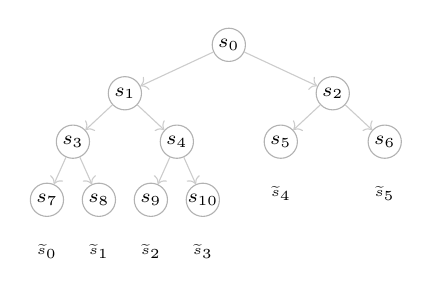
\begin{tikzpicture}[x=0.66cm, y=0.82cm]
  \tikzstyle{neutnode}  = [circle, draw=gray!60, fill=white, text=black, minimum size=12pt, inner sep=0pt, font=\scriptsize]
  \tikzstyle{treeedge} = [gray!40, rounded corners=2pt,->, thin]
  \tikzstyle{leaflbl}  = [font=\tiny, below=1pt]
  \node[neutnode](s0) at (3.5,0){$s_0$};
  \node[neutnode](s1) at (1.5,-.75){$s_1$};
  \node[neutnode](s2) at (5.5,-.75){$s_2$};
  \node[neutnode](s3) at (.5,-1.5){$s_3$};
  \node[neutnode](s4) at (2.5,-1.5){$s_4$};
  \node[neutnode](s5) at (4.5,-1.5){$s_5$};
  \node[neutnode](s6) at (6.5,-1.5){$s_6$};
  \node[neutnode](s7) at (0,-2.4){$s_7$};
  \node[neutnode](s8) at (1,-2.4){$s_8$};
  \node[neutnode](s9) at (2,-2.4){$s_9$};
  \node[neutnode](s10) at (3,-2.4){$s_{10}$};
  \node[leaflbl] at (0,-2.9){$\eseed_0$};
  \node[leaflbl] at (1,-2.9){$\eseed_1$};
  \node[leaflbl] at (2,-2.9){$\eseed_2$};
  \node[leaflbl] at (3,-2.9){$\eseed_3$};
  \node[leaflbl] at (4.5,-2.0){$\eseed_4$};
  \node[leaflbl] at (6.5,-2.0){$\eseed_5$};
  \draw[treeedge](s0)--(s1);\draw[treeedge](s0)--(s2);
  \draw[treeedge](s1)--(s3);\draw[treeedge](s1)--(s4);
  \draw[treeedge](s2)--(s5);\draw[treeedge](s2)--(s6);
  \draw[treeedge](s3)--(s7);\draw[treeedge](s3)--(s8);
  \draw[treeedge](s4)--(s9);\draw[treeedge](s4)--(s10);
  
\end{tikzpicture}
\vspace{2pt}
{\small (a) Expanded reference \GGM\ seed tree.}
\end{minipage}%
\hfill%
\begin{minipage}[b]{0.55\linewidth}
\centering
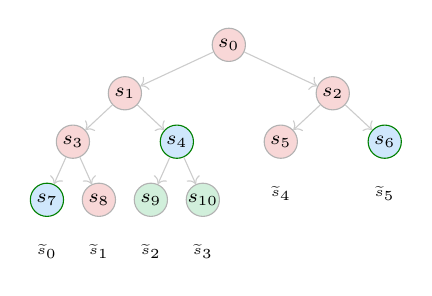
\begin{tikzpicture}[x=0.66cm, y=0.82cm]
  \tikzstyle{neutnode} = [circle, draw=gray!60, fill=nodehid, text=black, minimum size=12pt, inner sep=0pt, font=\scriptsize]
  \tikzstyle{pubnode}  = [circle, draw=green!50!black, fill=nodepath, minimum size=12pt, inner sep=0pt, font=\scriptsize]
  \tikzstyle{zeronode} = [circle, draw=gray!60, fill=nodepub, minimum size=12pt, inner sep=0pt, font=\scriptsize]
  \tikzstyle{treeedge} = [gray!40, rounded corners=2pt,->, thin]
  \tikzstyle{leaflbl}  = [font=\tiny, below=1pt]
  \node[neutnode](s0) at (3.5,0){$s_0$};
  \node[neutnode](s1) at (1.5,-.75){$s_1$};
  \node[neutnode](s2) at (5.5,-.75){$s_2$};
  \node[neutnode](s3) at (.5,-1.5){$s_3$};
  \node[pubnode] (s4) at (2.5,-1.5){$s_4$};
  \node[neutnode](s5) at (4.5,-1.5){$s_5$};
  \node[pubnode] (s6) at (6.5,-1.5){$s_6$};
  \node[pubnode] (s7) at (0,-2.4){$s_7$};
  \node[neutnode](s8) at (1,-2.4){$s_8$};
  \node[zeronode](s9) at (2,-2.4){$s_9$};
  \node[zeronode](s10) at (3,-2.4){$s_{10}$};
  \node[leaflbl] at (0,-2.9){$\eseed_0$};
  \node[leaflbl] at (1,-2.9){$\eseed_1$};
  \node[leaflbl] at (2,-2.9){$\eseed_2$};
  \node[leaflbl] at (3,-2.9){$\eseed_3$};
  \node[leaflbl] at (4.5,-2.0){$\eseed_4$};
  \node[leaflbl] at (6.5,-2.0){$\eseed_5$};
  \draw[treeedge](s0)--(s1);\draw[treeedge](s0)--(s2);
  \draw[treeedge](s1)--(s3);\draw[treeedge](s1)--(s4);
  \draw[treeedge](s2)--(s5);\draw[treeedge](s2)--(s6);
  \draw[treeedge](s3)--(s7);\draw[treeedge](s3)--(s8);
  \draw[treeedge](s4)--(s9);\draw[treeedge](s4)--(s10);
  
\end{tikzpicture}
\vspace{2pt}
{\small (b) After \Chal, \Decide, \Publish; $\mathbf{b}\!=\!\{0,1,0,0,1,0\}$, $\tpath\!=\!\{s_4,s_6,s_7\}$.}
\end{minipage}
\caption{GGM seed tree ($t=6$): structure~(a) and flag state~(b).
In~(b): pink nodes ($\calF{=}1$, hidden subtree); green nodes ($\calF{=}0$,
fully revealed subtree); blue-bordered nodes ($\calF{=}0$, in $\tpath$).}
\label{fig:less-trees}
\end{figure}


\subsection{The faulted oracle and dual revelation}
\label{sec:oracle}

\begin{definition}[Faulted Signing Oracle]
\label{def:fault-oracle}
Let $\Pi=(\Setup,\Expand,\Chal,\Decide,\allowbreak
\Publish,\allowbreak\Recon)$ be a \GZKST
instance, let $\Sig[\Pi]$ be the derived signature scheme of
Definition~\ref{def:sigma}, and let $(\sk,\pk)$ be a fixed key pair. For a
node $v^*\in V(\calT)$, the oracle $\Oracle^{v^*}(\sk,\pk)$ runs
$\Sig[\Pi].\Sign(\sk,\msg)$ unmodified except that, during
$\Publish(\calT,\calH)$, it forces
$\calF(v^*) \leftarrow 0$
before the normal upward propagation step. The oracle outputs the
resulting (possibly faulted) signature $\sig^*$.
\end{definition}

A fault is \emph{effective} if $v^*$ originally satisfies
$\calF(v^*)=1$ and is an ancestor of some hidden leaf
$\eseed_i$ with $i\in\calH$. In this case, the published path
reveals a node from which $\eseed_i$ is derivable, violating
Invariant~\ref{inv:hiding}. Otherwise, the fault is
\emph{ineffective}.

Definition~\ref{def:fault-oracle} is realised by instruction skips,
stuck-at-zero faults, bit flips and clock
glitches~\cite{ZKFault,FaultToForge2025} alike; the abstraction is indifferent
to which. An honest signature reveals $\resp_i$ for every $i \in \calH$ while
keeping $\eseed_i$ hidden, and an effective fault breaks that separation,
handing the attacker both. We call this \emph{dual revelation}; it is the
primitive underlying every secret-recovery attack in this work.






\subsection{A taxonomy of fault surfaces}
\label{sec:taxonomy}

The value of Definitions~\ref{def:gzkst} and~\ref{def:sigma} is not that they
restate the (obvious) fact that revealing a hidden seed breaks zero knowledge.
It is that they make the fault surface \emph{enumerable}. Every implementation
of $\Sig[\Pi]$ must materialise each of the components in turn, and each
component admits its own class of faults with its own consequence:

\begin{itemize}[leftmargin=*,itemsep=1pt]
  \item $\Setup$: biasing or zeroing $\seed_r$ makes the whole tree, and hence
        every $\eseed_i$, predictable without touching $\Publish$.
  \item $\Expand$: skipping a \PRG\ invocation leaves a child at a known or
        stale value --- the surface exploited against
        FAEST~\cite{JendralD25} and Mirath/RYDE~\cite{BandaBK26}.
  \item $\Chal$: corrupting the digest before parsing changes which rounds are
        hidden; the attack of~\cite{HuangHHYSTY26} skips iterations of the
        digest-preprocessing loop of LESS-v2 and never touches the tree.
  \item $\Decide$: forcing $c_i \leftarrow 0$ moves a round from $\calH$ to
        $\calR$, so its seed is published \emph{legitimately} after $\resp_i$
        has already been emitted.
  \item $\Publish$: corrupting the per-node release decision ---
        \cite{ZKFault,FaultToForge2025} and all three attacks of
        Section~\ref{sec:app}.
  \item $\Recon$: verifier-side, so relevant to acceptance rather than key
        recovery; it matters here because a verify-before-release
        countermeasure runs $\Recon$ on the signer's own device
        (Section~\ref{sec:counter}).
\end{itemize}

Table~\ref{tab:surfaces} places the published attacks on this grid. Two
observations follow. First, five independent attacks developed against four
schemes, with different tree shapes and different secret types, occupy only
three of the six components, which suggests the grid is the right coordinate
system rather than an artefact. Second, the empty cells are predictions: one
of them produced Model~2 of Section~\ref{sec:app}, since asking what
\emph{else} inside $\Publish$ can be faulted besides the flag value points at
the index bookkeeping that walks the tree --- a surface with no analogue in the
LESS flag array, and one no previous work had considered.

\begin{table}[htbp]
\centering
\caption{Published fault attacks on \GZKST-based signatures, classified by the
component of Definitions~\ref{def:gzkst}--\ref{def:round} that the fault
corrupts.}
\label{tab:surfaces}
\resizebox{\textwidth}{!}{
\setlength{\tabcolsep}{4pt}
\begin{tabular}{@{}llll@{}}
\toprule
\textbf{Work} & \textbf{Target scheme(s)} & \textbf{Component} & \textbf{Outcome} \\
\midrule
ZKFault~\cite{ZKFault}                & LESS-v1, CROSS   & \Publish          & key recovery \\
Fault to Forge~\cite{FaultToForge2025} & LESS-v2          & \Publish          & universal forgery \\
Faultless key recovery~\cite{HuangHHYSTY26} & LESS-v2     & \Chal             & key recovery \\
Fault attack on MPCitH~\cite{BandaBK26} & Mirath, RYDE    & \Expand, \Chal    & key recovery, forgery \\
Case study on FAEST~\cite{JendralD25}  & FAEST            & \Expand           & key recovery \\
\midrule
This work (Section~\ref{sec:app})      & MEDS             & \Publish ($3$ surfaces) & key recovery \\
\bottomrule
\end{tabular}
}paper
\end{table}

\begin{remark}[Specification versus implementation]
\label{rem:spec-vs-impl}
One scheme may realise a component in two inequivalent ways. The MEDS
specification~\cite{MEDS_PQC} describes $\Publish$ as bottom-up OR-propagation
followed by depth-first serialisation of the boundary; the reference
implementation performs a depth-first descent driven by an index cursor into
the sorted hidden-leaf list, with no flag array at all. Both satisfy
Invariants~\ref{inv:correctness} and~\ref{inv:hiding}, yet their fault
surfaces are disjoint. Analysing the abstraction alone is therefore not
enough, and one implementation does not transfer to another;
Section~\ref{sec:app} attacks the implementation.
\end{remark}

\subsection{Secret extraction and key recovery}
\label{sec:extract}

Extraction is the inverse of $\Resp$ once the leaf seed is known:

\begin{definition}[Extract]
\label{def:extract}
$\Extract(\eseed_i, \resp_i, \pk) \to \sk'$: given the leaked seed
$\eseed_i$ and the ZK response $\resp_i$ for the same round $i \in \calH$,
recover the (partial) secret $\sk' \subseteq \calS$.
\end{definition}

Equivalently, $\Extract$ inverts $\Resp$ once its first argument is known,
and in every scheme considered here it is linear algebra. For MEDS, a hidden
round with $h_i = j$ publishes $(\mu_i,\nu_i)$ as in~\eqref{eq:meds-resp};
expanding $\eseed_i$ gives $(\tilde{A}_i,\tilde{B}_i)$ and hence
$A_j^{-1} = \tilde{A}_i^{-1}\mu_i$ and $B_j^{-1} = \nu_i \tilde{B}_i^{-1}$ by
two inversions and two products over $\Fq$. For CROSS the response encodes
$\mathbf{v}_i = \mathbf{e} \star (\mathbf{e}'_i)^{-1}$, so
$\mathbf{e} = \mathbf{v}_i \star \mathbf{e}'_i$ directly. For LESS-v2 the
response is a coset representative and $\pi_{b[i]}$ follows from the
column-extraction argument of Lemma~1 in~\cite{FaultToForge2025}.

\noindent\textbf{Full key recovery.}
When $|\calS| = s-1 > 1$ a single effective fault recovers only the secret
indexed by $h_i$, so full recovery is a coupon-collector problem over
$j \in \{1,\ldots,s-1\}$.

\begin{algorithm}[tb]
\caption{GZKST key recovery from faulted oracle}
\label{alg:key-recovery}
\SetKwInOut{Input}{Input}
\SetKwInOut{Output}{Output}
\Input{Faulted oracle $\Oracle^{v^*}$, public key $\pk$}
\Output{Recovered secret key $\widehat{\sk}$}
$\mathsf{Collected} \leftarrow \emptyset$\;
\While{$|\mathsf{Collected}| < |\calS|$}{
  $\sig^* \leftarrow \Oracle^{v^*}(\msg)$ for an arbitrary $\msg$\;
  \If{$\sig^*$ is \emph{effective}}{
    \For{each $i \in \mathsf{leaked}(\sig^*)$}{
      $\sk' \leftarrow \Extract\!\left(\eseed_i,\, \resp_i,\, \pk\right)$\;
      $\mathsf{Collected} \leftarrow \mathsf{Collected} \cup \{(j, \sk')\}$
        where $j = c_i$\;
    }
  }
}
\Return $\widehat{\sk} \leftarrow \mathsf{Collected}$\;
\end{algorithm}

\begin{proposition}[Correctness and query complexity]
\label{prop:alg-correctness}
Let $\Pi$ be a \GZKST\ instance, let $v^* = \mathrm{root}$ so that the fault
exposes all $w$ hidden leaves and $L = w$ is deterministic, and put
$p_{\min} = 1 - \bigl(\tfrac{s-2}{s-1}\bigr)^{w}$. Then
Algorithm~\ref{alg:key-recovery} terminates with $\widehat{\sk} = \sk$, the
expected number of effective queries satisfies
$\mathbb{E}[Q] \leq (s-1)/p_{\min}$, and for any $\delta > 0$ at most
$\lceil \frac{s-1}{p_{\min}} \ln \frac{1}{\delta} \rceil$ effective queries
suffice with probability $1-\delta$. See Appendix~\ref{app:proof-recovery}.
\end{proposition}

For a fault at an arbitrary node the number of hidden leaves in its subtree is
hypergeometric and may fall below its mean, so $p_{\min}$ no longer bounds the
per-query success probability; the worst case of a single hidden leaf still
gives $\mathbb{E}[Q] \leq (s-1)H_{s-1} \leq 5H_5 \approx 11.4$. Deciding
whether a signature is effective is easy for the adversary: from the fault
location and the challenge, both recoverable from the signature, it recomputes
the honest flag tree and checks that $v^*$ was hidden and covers a hidden leaf.


The last two columns of Table~\ref{tab:scheme-params} instantiate this bound
for every MEDS parameter set. Because a root fault gives $\ell = t$ and hence
$L = w$ exactly, every set has $p_{\min} \geq 0.9966$ and therefore
$\mathbb{E}[Q] \leq s-1 \leq 5$: a handful of effective faults suffices at
every security level.


\noindent\textbf{From key recovery to forgery.}
On termination the adversary holds a complete signing key and can sign any
message, including ones never submitted to the oracle. This is a full break of
EUF-CMA.

\begin{corollary}
\label{cor:euf-cma}
Let $\Pi$ be a \GZKST-based signature scheme and let the fault model be as in
Definition~\ref{def:fault-oracle} (a stuck-at-zero perturbation of a single
flag bit during $\Publish$).  If an efficient adversary can induce this fault
at a fixed node $v^* \in V(\calT)$ on the victim's signing device, then
$\Pi$ is \emph{not} \textrm{EUF-CMA}-secure in the fault model: the adversary
recovers $\sk$ via Algorithm~\ref{alg:key-recovery} and forges signatures on
arbitrary messages without further oracle access.
\end{corollary}


\section{Fault Injection attacks on MEDS}
\label{sec:app}
We now attack the C reference implementation of MEDS,\footnote{\url{https://github.com/MEDSpqc/meds}}
exploiting the tree-traversal logic of the path construction --- \chg{line~\ref{alg:meds:path}} of
Algorithm~\ref{alg:sign_meds} --- to leak hidden seeds. In that
implementation, path generation and tree reconstruction are not two functions
but two modes of one, \texttt{stree\_to\_path\_to\_stree}, selected by a
\texttt{mode} parameter; Listing~\ref{lst:path} gives the traversal.

\begin{lstlisting}[style=cstyle,caption={Traversal loop of \texttt{stree\_to\_path\_to\_stree}; highlights mark the three fault targets.},label=lst:path]
void stree_to_path_to_stree(uint8_t *stree, ..., uint8_t *path, int mode) {
    while (1==1) {
        int index_leaf = 0;
        `\label{lst:path:while}\highlight{yhl}{while ((indices[id] \chg{>{}>} (MEDS\_seed\_tree\_height-h)) == i)}` 
        {// Traverse down toward the secret leaf
            h += 1;
            i <<= 1;
            if (h > MEDS_seed_tree_height) {
                h -= 1;
                i >>= 1;
                `\label{lst:path:inc}\highlight{rhl}{if (id + 1 < MEDS\_w) id++; }`
                `\label{lst:path:leaf}\highlight{bhl}{index\_leaf = 1;}` // Flag node as hidden
                break;
            }
        }
        ...
    }
}
\end{lstlisting}

The algorithm identifies the secret leaves ($h[i] > 0$) and performs a
depth-first search, halting as soon as it reaches a node that is no longer an
ancestor of the current hidden leaf and appending that node to the path. On
reaching a hidden leaf it sets \texttt{index\_leaf}, so the leaf seed stays
unpublished, and moves to the next one.

Our objective is to manipulate the control flow so that unpublished seeds ---
internal nodes or leaves --- are written into the public signature path.

\paragraph{Threat model and what a successful fault yields.}
\revon
Our \emph{intended} attack scenario is a victim device that signs a requested
message and emits the resulting output despite a fault. The experiments
below instead glitch a standalone invocation of the publication routine,
using a fixed tree, salt and challenge; no full signing operation is run.
In the intended attack, the adversary does \emph{not} need the
emitted signature to be valid, a point that matters for
\revoff
Section~\ref{sec:counter}: $\resp_i = (\mu_i,\nu_i)$ is present for every
hidden round regardless of the fault, so once the corrupted path discloses
$\sigma_i$ for one such round the extraction of~\eqref{eq:meds-extract}
succeeds even if the digest check would reject. What the adversary needs is
not a valid signature but an \emph{emitted} one.

\paragraph{Experimental Setup.}
Our experimental platform consists of a CW303-STM32F3 target board carrying an
ARM Cortex-M4 STM32F303RCT7 processor. Clock glitching is
performed using a ChipWhisperer-Lite.

\revon
\paragraph{Experimental scope.}
The board executes only the seed-path routine with fixed tree, salt and
challenge. Locating the vulnerable instruction after a complete signing
operation, producing a serialized faulted signature and recovering secret
components on-device were not tested. Thus the measured routine-level yields
cannot be read as end-to-end attack probabilities. Other hardware fault work
on this family has likewise isolated subfunctions~\cite{BandaBK26}.
\revoff

%\subsection{Fault Models}
\paragraph{Fault Models.}
We propose three fault models targeting different stages of the tree traversal.

\noindent\textbf{Model 1: Full Tree Recovery (Root Leakage).}
This attack aims to reveal the root seed, which effectively compromises the entire tree. By injecting a fault that causes the skip of the first iteration of \highlight{yhl}{\texttt{while} loop} at \chg{line~\ref{lst:path:while}} of Listing~\ref{lst:path}, the DFS halts immediately at the root ($h=0, i=0$). The root is incorrectly identified as a node ready for publication.

\noindent\textit{Detection and recovery.} The signature path contains only a
single non-zero element. The adversary confirms the fault offline by expanding
that seed into a full tree, recomputing the round commitments, and checking
them against the digest $d$ carried in the signature; no interaction with the
device is required. Note that the resulting path does not deserialise
correctly under an honest $\PathToSeedTree_t$, so this fault is detectable by
the signer --- see Section~\ref{sec:counter}.

\noindent\textbf{Model 2: Subtree Recovery.}
By glitching the guarded increment \highlight{rhl}{\texttt{id++}} at \chg{line~\ref{lst:path:inc}}
of Listing~\ref{lst:path}, the algorithm fails to advance the cursor
\texttt{id} into the list of hidden leaves. The traversal logic becomes desynchronized, resulting in the algorithm treating subsequent branches as public. All leaves to the right of the faulted \texttt{id} become computable.

\noindent\textit{Detection and recovery.} This fault is harder to recognise
than the other two, since the path has a plausible length. The adversary can
nonetheless simulate the reconstruction for each of the $w$ possible faulted
values of \texttt{id} and keep the one whose recomputed commitments match $d$,
at a cost of at most $w$ verifications.

\begin{figure}[!tb]
\centering
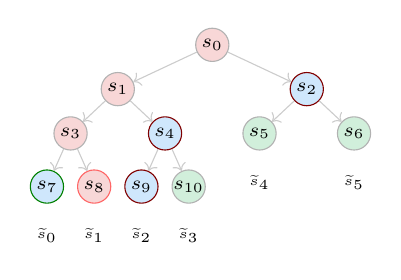
\begin{tikzpicture}[x=0.6cm, y=0.75cm]
  \tikzstyle{neutnode} = [circle, draw=gray!60, fill=nodehid, text=black, minimum size=12pt, inner sep=0pt, font=\scriptsize]
  \tikzstyle{faulted_leaf} = [circle, draw=red!60, fill=nodehid, text=black, minimum size=12pt, inner sep=0pt, font=\scriptsize]
  \tikzstyle{pubnode}  = [circle, draw=green!50!black, fill=nodepath, minimum size=12pt, inner sep=0pt, font=\scriptsize]
  \tikzstyle{fpubnode}  = [circle, draw=red!50!black, fill=nodepath, minimum size=12pt, inner sep=0pt, font=\scriptsize]
  \tikzstyle{zeronode} = [circle, draw=gray!60, fill=nodepub, minimum size=12pt, inner sep=0pt, font=\scriptsize]
  \tikzstyle{treeedge} = [gray!40, rounded corners=2pt,->, thin]
  \tikzstyle{leaflbl}  = [font=\tiny, below=1pt]
  \node[neutnode](s0) at (3.5,0){$s_0$};
  \node[neutnode](s1) at (1.5,-.75){$s_1$};
  \node[fpubnode](s2) at (5.5,-.75){$s_2$};
  \node[neutnode](s3) at (.5,-1.5){$s_3$};
  \node[fpubnode] (s4) at (2.5,-1.5){$s_4$};
  \node[zeronode](s5) at (4.5,-1.5){$s_5$};
  \node[zeronode] (s6) at (6.5,-1.5){$s_6$};
  \node[pubnode] (s7) at (0,-2.4){$s_7$};
  \node[faulted_leaf](s8) at (1,-2.4){$s_8$};
  \node[fpubnode](s9) at (2,-2.4){$s_9$};
  \node[zeronode](s10) at (3,-2.4){$s_{10}$};
  \node[leaflbl] at (0,-2.9){$\eseed_0$};
  \node[leaflbl] at (1,-2.9){$\eseed_1$};
  \node[leaflbl] at (2,-2.9){$\eseed_2$};
  \node[leaflbl] at (3,-2.9){$\eseed_3$};
  \node[leaflbl] at (4.5,-2.0){$\eseed_4$};
  \node[leaflbl] at (6.5,-2.0){$\eseed_5$};
  \draw[treeedge](s0)--(s1);\draw[treeedge](s0)--(s2);
  \draw[treeedge](s1)--(s3);\draw[treeedge](s1)--(s4);
  \draw[treeedge](s2)--(s5);\draw[treeedge](s2)--(s6);
  \draw[treeedge](s3)--(s7);\draw[treeedge](s3)--(s8);
  \draw[treeedge](s4)--(s9);\draw[treeedge](s4)--(s10);
\end{tikzpicture}
\caption{Effect of fault model 2 on the example presented in Figure~\ref{fig:less-trees}, if the glitch \chg{occurred while \texttt{id==0}, i.e.\ at the first hidden leaf $\eseed_1$ (at \texttt{id==1} the guarded increment is already a no-op for $w=2$)}. The returned path is $\{s_7,s_9,s_4,s_2\}$ and all leaves are computable except $\eseed_1$.}
\label{fig:faulted_path}
\end{figure}

\noindent\textbf{Model 3: Hidden Leaf Recovery.}
This model targets the specific instruction \highlight{bhl}{\texttt{index\_leaf = 1;}} at \chg{line~\ref{lst:path:leaf}} of Listing~\ref{lst:path}. By skipping this assignment, a hidden leaf is no longer marked as private. The execution continues normally, but the secret leaf seed is copied into the \texttt{path} buffer.

\noindent\textit{Detection and recovery.} \chg{The path carries $k > 0$ extra
seeds, one per skipped assignment, so it is $k$ entries longer than the honest
path, whose length the adversary computes from $\mathbf{h}$. No subset search
is needed to exploit it: for each path entry $\sigma$ and each hidden round
$i$, the adversary expands $\sigma$ as the round-$i$ seed, extracts a candidate
$(A_j^{-1},B_j^{-1})$ with $j = h_i$ by~\eqref{eq:meds-extract}, and keeps it
if $\SF(\pimap{A_j}{B_j}(G_0)) = G_j$. This costs at most $w\cdot|\tpath|$
such tests, each a handful of matrix operations over $\Fq$.}

\chg{\noindent\textit{Relation to Definition~\ref{def:fault-oracle}.} The
reference implementation has no flag array, but Models~1 and~3 have the effect
of the faulted oracle: Model~1 publishes the root, as $\Oracle^{\mathrm{root}}$
does, so Proposition~\ref{prop:alg-correctness} applies with $L = w$; Model~3
publishes a single hidden leaf, as $\Oracle^{v^*}$ does with $v^*$ that leaf
($L = 1$, the $(s-1)H_{s-1}$ case of Section~\ref{sec:extract}). Model~2
corrupts the cursor rather than one node's release decision, so it is not an
instance of Definition~\ref{def:fault-oracle}; it exposes the hidden leaves
\revon
to the right of the faulted position, so $1 \leq L \leq w$ for useful disclosures. Neither its empirical
$L$ distribution nor an end-to-end recovery rate was measured.}
\revoff

\subsection{Results}

\revon
We reproduced all three targeted faulty path outputs on a
ChipWhisperer-Lite/STM32F303 testbed. 
\revoff

\revon
We bracket the instruction under test with GPIO triggers and check the
disassembly for trigger placement. After tuning the glitch duration, we
sweep \texttt{width} (pulse width), \texttt{offset} (phase) and
\texttt{ext\_offset} (cycles after the trigger). This arrangement gives
instruction-level synchronization unavailable from the beginning of a full
signing request.
\revoff


\chg{
  We separate exploration from confirmation. A coarse sweep of the
\texttt{ext\_offset}, \texttt{offset} and \texttt{width} grid at $10$ attempts
per point locates the vulnerable region; we then fix the single highest-yield
point and re-run $100$ \emph{independent} attempts there, and it is these
confirmatory runs that Table~\ref{tab:fault-success} reports, as
$p_{\mathrm{best}}$ with a Wilson $95\%$ confidence interval and the reset
rate. The vulnerable window is narrow: across the full swept grid only a small
fraction of points fault at all (e.g.\ $33$ of $672$ for Model~1, $4$ of $448$
for Model~3), so the grid-averaged yield is one to two orders of magnitude
\revon
below $p_{\mathrm{best}}$. Proposition~\ref{prop:alg-correctness} applies to \emph{root
disclosure only}. The inverse calibrated success probability $1/p_{\mathrm{best}}$
is the geometric mean number of routine invocations to obtain the specified
target output, if repeated attempts are independent. It excludes the initial
parameter search, resets, timing uncertainty of full signing and, for
Models~2--3, the further disclosures needed to recover all components. All runs use a core clock of $7.37$\,MHz.}
\revoff


\begin{table}[htp]
\centering
\caption{\chg{Single-glitch outcome rates at the best parameter point, from
$100$ independent confirmatory attempts (the \textbf{att.}\ column).
$p_{\mathrm{best}}$ is given with a Wilson $95\%$ confidence interval, alongside
\revon
the reset rate and the idealised mean
invocations $1/p_{\mathrm{best}}$ needed for the specified target output.
These are \emph{not} end-to-end signing-request or full-key recovery costs. The best-point
\revoff
$(\texttt{ext\_offset},\texttt{offset},\texttt{width})$ settings are stated per
model in the text; the success-map figures sweep the full grid at $10$ attempts
per point.}}
\label{tab:fault-success}
\setlength{\tabcolsep}{5pt}
\small
\begin{tabular}{@{}l|l|r|r|c|r|r@{}}
\toprule
\textbf{Model} & \textbf{Opt.} & \textbf{att.} & $p_{\mathrm{best}}$ &
\chg{\textbf{95\% CI}} & \textbf{reset} & \rev{\chg{\textbf{inv./hit}}} \\
\midrule
1 (root)        & \texttt{-Os} & $100$ & $0.85$ & \chg{$[0.77,0.91]$} & $0.01$ & \rev{$1.18$} \\
\midrule
2 (subtree)     & \texttt{-Os} & $100$ & $0.23$ & \chg{$[0.16,0.32]$} & $0.62$ & \rev{$4.35$} \\
\midrule
3 (hidden leaf) & \texttt{-O0} & $100$ & $0.16$ & \chg{$[0.10,0.24]$} & $0.05$ & \rev{$6.25$} \\
\bottomrule
\end{tabular}
\end{table}

\chg{\paragraph{Reproducibility.} We collect the settings in one place. The
device is a CW303 STM32F303RCT7 (ARM Cortex-M4) on a ChipWhisperer-Lite, core
clock $7.37$\,MHz, driven over SimpleSerial~v2.1. The target is the
\texttt{stree\_to\_path\_to\_stree} routine of the MEDS reference
\revon
implementation for a single parameter set, one MEDS level-I configuration (tree height
\revoff
$\lceil\log_2 t\rceil$, $w$ hidden rounds), built with \texttt{arm-none-eabi-gcc}
through the ChipWhisperer makefile, with \texttt{PLATFORM=CWLITEARM} and
\texttt{GLITCH\_MODEL=}$m$. Models~1 and~2 use the project default
\texttt{-Os}; Model~3
forces only its target function to \texttt{-O0}
(via a GCC \texttt{optimize} function attribute), the rest of the image staying
at \texttt{-Os} so it still fits flash. The clock-glitch sweep ranges over
\texttt{ext\_offset} ($0$--$11$ for Model~1, $0$--$46$ in steps of $2$ for
Model~2, $0$--$7$ for Model~3), \texttt{offset} ($\pm4$, excluding $0$) and
\texttt{width} ($4$--$10$), giving $672$, $1344$ and $448$ grid points and $10$
attempts per point. The maximum-yield point is then re-measured with $100$
independent attempts, disjoint from the sweep; these are the figures of
Table~\ref{tab:fault-success}. The exact parameter set, the
\texttt{arm-none-eabi-gcc} version and the source commit are pinned in the
accompanying artefact, with the harness (\texttt{cw\_meds\_glitch.py}) and the
instrumented \texttt{seed.c}.}

\textbf{Model 1: Full tree recovery.}
This attack is successful if the returned path contains a
single node which is the root node.

\textit{Compilation.} This attack is carried out on a 
code compiled with the default \texttt{-Os} optimization.

\textit{Trigger position.} We directly target the 
evaluation of the conditional and the branching 
instruction corresponding to \chg{line~\ref{lst:path:while}} of Listing~\ref{lst:path}. 
The compiled result is Listing~\ref{lst:f1asm} in
Appendix~\ref{app:asm}; we fault for three clock cycles.

\textit{Parameters.} \chg{The best point is \texttt{ext\_offset}$=9$,
\texttt{offset}$=3$, \texttt{width}$=9$, giving $85\%$ success over $100$
attempts with a $1\%$ reset rate; the hot band spans \texttt{ext\_offset}
$7$--$9$. Figure~\ref{fig:fault1_results} maps the outcomes and the rates are
the Model~1 row of Table~\ref{tab:fault-success}.}

\begin{figure}[!tb]
\centering
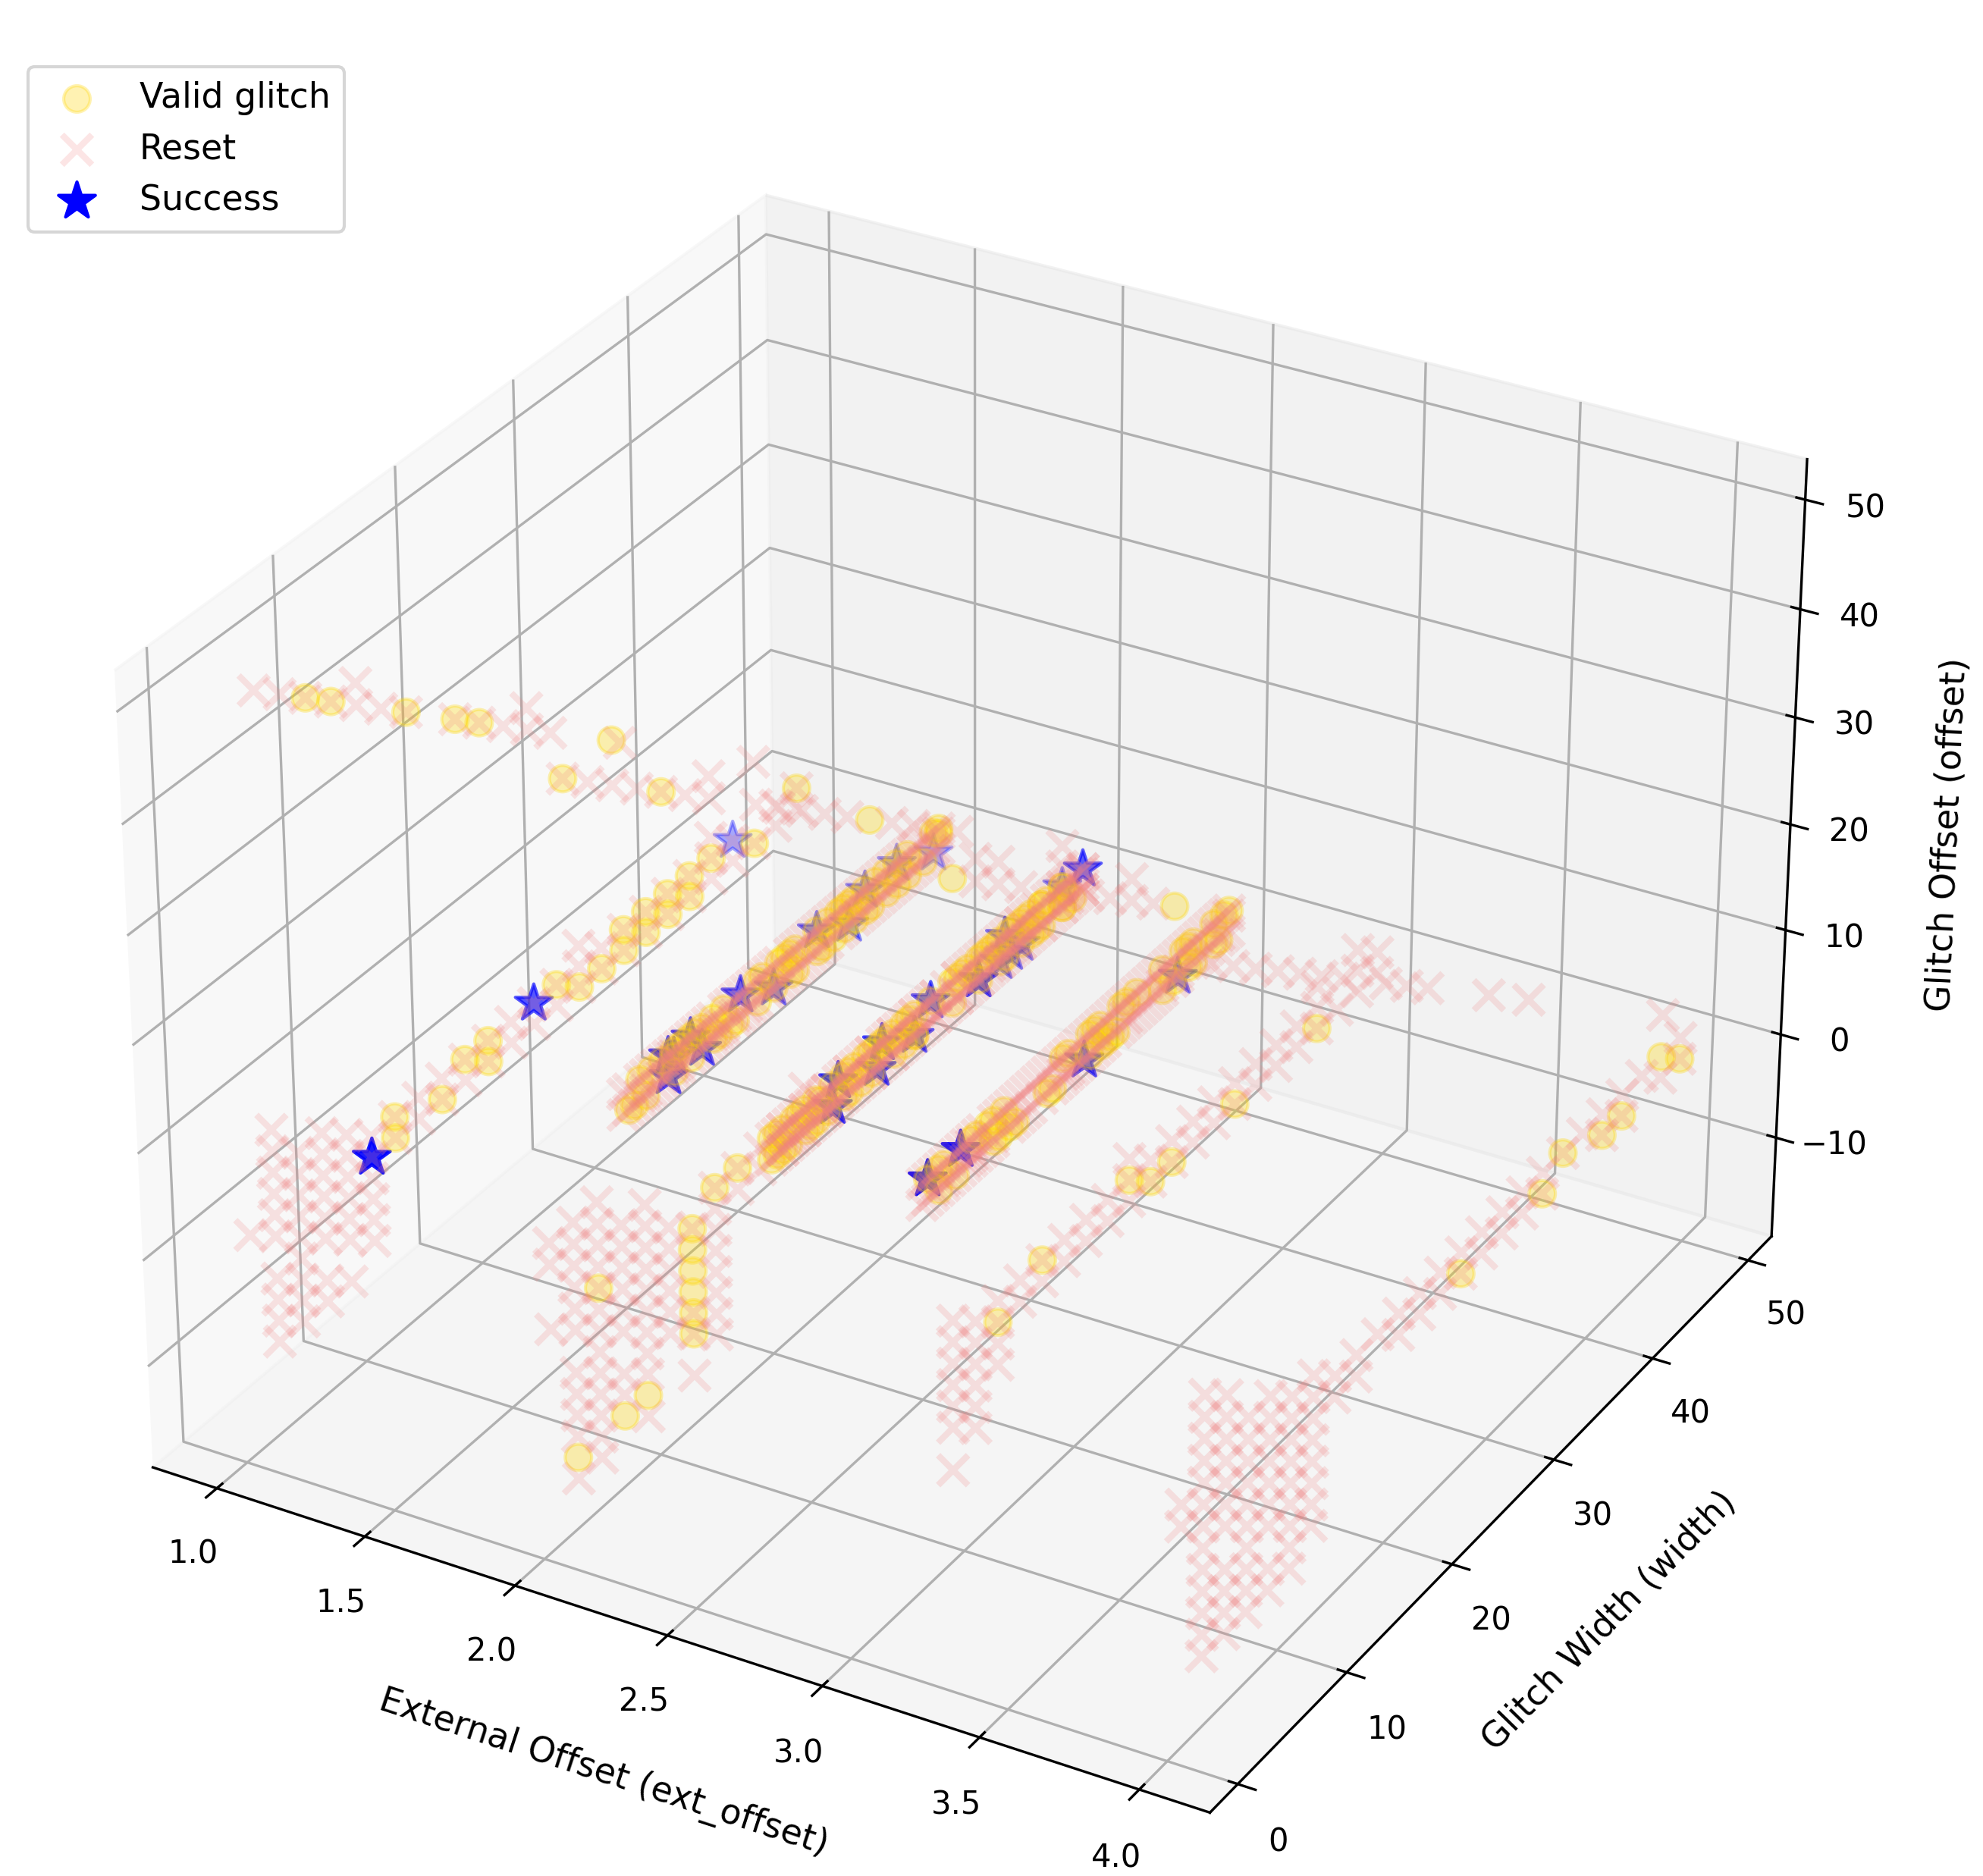
\includegraphics[width=0.56\textwidth]{content/images/glitch_3d_results_crop.png}
\caption{Model 1 (full tree disclosure): glitch outcome over
\texttt{ext\_offset}, \texttt{width} and \texttt{offset}, $10$ attempts per
parameter point. Blue stars mark successful faults, yellow circles
\emph{valid} glitches (runs that neither crashed nor produced the correct or
the target faulted path), pink crosses device resets.}
\label{fig:fault1_results}
\end{figure}

\textbf{Model 2: Subtree recovery.} We consider 
this attack successful if we obtain the faulted path pattern 
described by Figure~\ref{fig:faulted_path}. 

\textit{Compilation.} This is carried out on a code compiled with the default \texttt{-Os} optimization.

\textit{Trigger position.} The trigger frames \chg{line~\ref{lst:path:inc}} of
Listing~\ref{lst:path}; the compiled result is Listing~\ref{lst:f2asm} in
Appendix~\ref{app:asm}.

\textit{Parameters.} Evaluating the condition and incrementing \texttt{id}
take $3$ clock cycles, so we set \texttt{repeat} to $3$;
Figure~\ref{fig:fault2_results} gives the resulting success map. \chg{The best
point is \texttt{ext\_offset}$=2$, \texttt{offset}$=4$, \texttt{width}$=9$,
giving $23\%$ success over $100$ confirmatory attempts (Wilson $95\%$ CI
$[16\%,32\%]$) with a $62\%$ reset rate; these are the Model~2 row of
Table~\ref{tab:fault-success}.}

For Model~2 we observe a bounded region of system resets bordered by
successful attacks and other valid glitches, many of whose paths carry enough
intermediate nodes to recompute every leaf.

\textbf{Model 3: Single hidden leaf recovery.} Here only one hidden leaf is
disclosed.

\textit{Compilation.} At \texttt{-O1} and above, including \texttt{-Os}, the
compiler removes the explicit assignment and achieves the same outcome through
control flow, leaving nothing precise to target. We therefore build the target
function at \texttt{-O0}; applying \texttt{-O0} project-wide overflows the
board's flash.

\textit{Trigger position.} On the unoptimised build we place the high trigger
immediately before the \texttt{index\_leaf} assignment and the low trigger
immediately after; the compiled result is Listing~\ref{lst:f3asm} in
Appendix~\ref{app:asm}.

\textit{Parameters.} The disassembly shows the assignment compiled to two
single-cycle instructions, so we set \texttt{repeat} to $2$;
Figure~\ref{fig:fault3_results} gives the success map. \chg{The best point is
\texttt{ext\_offset}$=7$, \texttt{offset}$=3$, \texttt{width}$=8$, giving
$16\%$ success over $100$ confirmatory attempts (Wilson $95\%$ CI
$[10\%,24\%]$) with a $5\%$ reset rate; the hot band is confined to
\texttt{ext\_offset}$=7$.}

\begin{figure}[!tb]
\centering
\begin{subfigure}[b]{0.46\textwidth}
  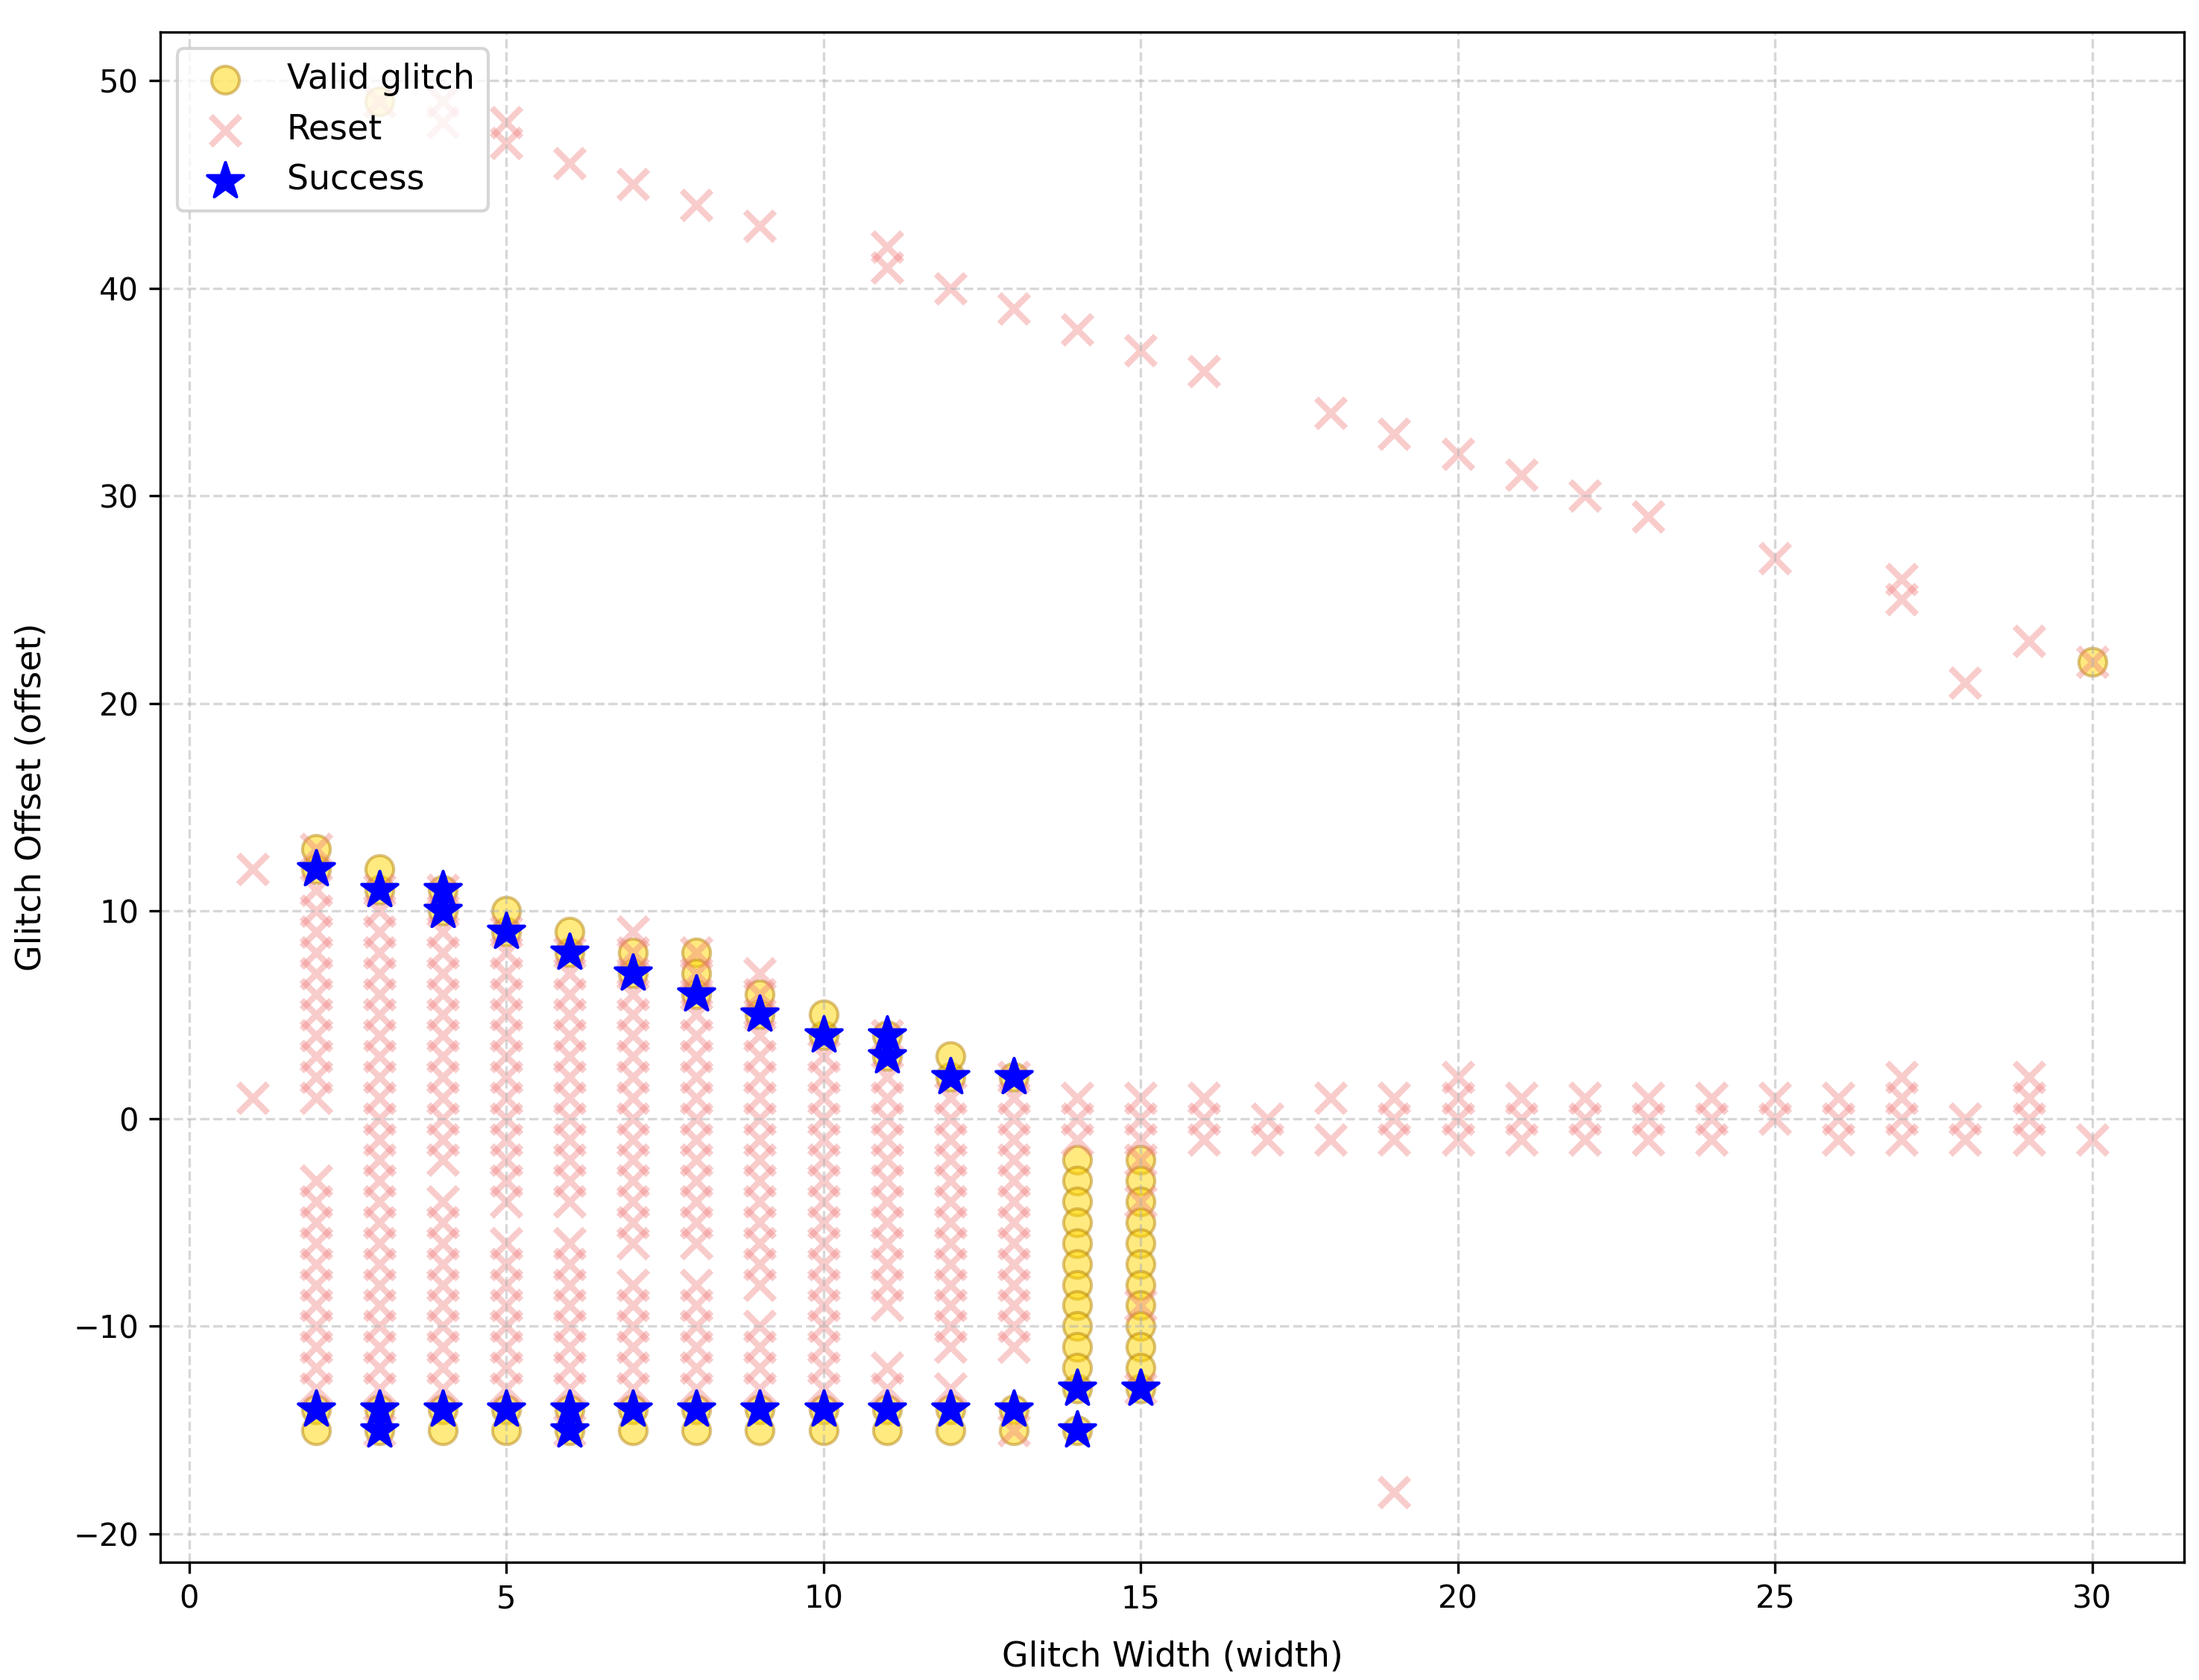
\includegraphics[width=\linewidth]{content/images/glitch_2d_results_ext2_crop.png}
  \caption{Model 2 (subtree), $\texttt{ext\_offset} = 2$.}
  \label{fig:fault2_results}
\end{subfigure}\hfill
\begin{subfigure}[b]{0.46\textwidth}
  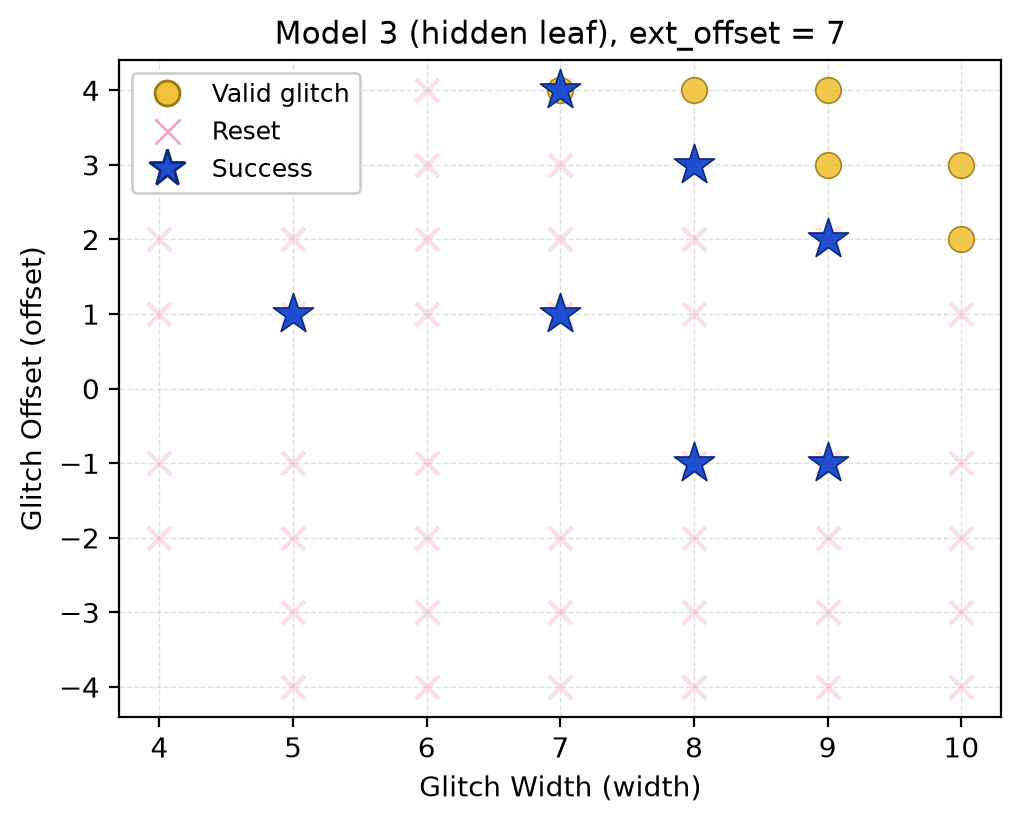
\includegraphics[width=\linewidth]{content/images/glitch_2d_results_ext7_crop.png}
  \caption{\chg{Model 3 (hidden leaf), $\texttt{ext\_offset} = 7$.}}
  \label{fig:fault3_results}
\end{subfigure}
\caption{Glitch success frequency for Models~2 and~3, $10$ attempts per
parameter point; markers as in Figure~\ref{fig:fault1_results}.}
\label{fig:glitch_results}
\end{figure}

\revon
\noindent\textbf{Results.} The target faulty outputs are reproducible under instrumentation. \chg{For Model~3, every
\revoff
attempt} gave normal execution, a device reset, or the expected exploit, with
no other valid glitches --- a consequence of single-instruction targeting,
which is less likely than a wider disruption window to bleed into surrounding
cycles\chg{; Models~1 and~2 also produce other valid glitches
(Figures~\ref{fig:fault1_results} and~\ref{fig:fault2_results})}. Model~1, the root reveal, is both the most efficient and the most
reproducible; Models~2 and~3 replicate less readily but are harder to detect
\revon
during signing (Section~\ref{sec:counter}).
\noindent\textbf{Limits of the evidence.}
The rates in Table~\ref{tab:fault-success} describe tuned points selected
after searching $672$, $1344$ and $448$ parameter combinations (ten trials
per point), not success probabilities for a previously unprofiled device.
Only Model~1 yields the full-tree disclosure required by the one-query
coverage calculation; Models~2--3 generally expose fewer hidden seeds.
Our tests did not reconstruct MEDS response pairs from a full emitted
signature, demonstrate key extraction on the target, or measure the ability
to hit the publication routine from the start of complete signing. Model~3
uses a non-default \texttt{-O0} build, so its transfer to the normal
\texttt{-Os} binary remains open.
\revoff


\section{Countermeasures}
\label{sec:counter}
We now present countermeasures against the attacks above, in three
categories: \emph{post-publication path checks},
which preserve both the signature size and the tree construction;
\emph{modifications to the path-construction algorithm}, which preserve the
signature size but change how the path is produced; and \emph{tree-less
constructions}, which remove the mechanism entirely at a large cost in
signature size.


\paragraph{Post-publication path check.}

These run checks on the output of $\SeedTreeToPath$. A size check alone already
defeats fault models~1 and~3, whose paths have length $1$ and \chg{$|\tpath|+k$}
respectively \chg{($|\tpath|$ the honest length, $k \geq 1$ the number of leaked
leaves)}, and the expected size is computable from $\calH$ in linear time.
A stronger version rebuilds the tree with $\PathToSeedTree$ and compares the
recovered leaves against $\calH$ and the reference tree.

\noindent\textit{Verify-before-release, and why it is weaker than it looks.}
The most natural version of this countermeasure is the classical one: run the
verification algorithm on the signature before releasing it, and suppress the
output on mismatch. Against the attacks of Section~\ref{sec:app} this does
work in principle, because none of the three faulted paths deserialises to the
honest leaf set and the recomputed digest therefore differs from $d$.

It is weaker than it looks, for a structural reason. In the MEDS reference
code $\SeedTreeToPath$ and $\PathToSeedTree$ are two modes of one function
sharing the traversal loop of Listing~\ref{lst:path}, so the instruction the
attacker glitches during signing is \emph{the same instruction}, at the same
code offset, that the verification pass executes. An attacker who can place
one glitch can place two, and a ChipWhisperer emits both within a single
trace: the redundancy is nominal, since the check re-executes the faulted code
rather than checking it independently. \chg{The replayed glitch does not merely
break the check, it makes it pass: in reconstruction mode the same skip makes
the traversal consume the path exactly as the faulted construction produced
it. Under Model~1, for instance, $\PathToSeedTree$ with the same skip reads
the single published seed as the root, regenerates the whole tree, and returns
every revealed leaf correctly, so the recomputed digest equals $d$. For
Models~2 and~3 the second glitch must also hit the same iteration (the same
value of \texttt{id}).} This is why we prefer the decoupled construction below, and the point generalises --- any
implementation folding $\Publish$ and $\Recon$ into shared code inherits it.
We have not measured the double-glitch success rate, and doing so is the most
useful single extension of this work. Finally, note that such a countermeasure
must suppress the output entirely on detection rather than merely flag it:
as Section~\ref{sec:app} observes, the adversary needs an emitted corrupted
path, not a valid signature.



\paragraph{Decoupling path construction from the flag tree.}

Coupling flag-tree construction to path extraction is what makes the replay
above possible. Decoupling them into independent stages with a check after
each means a fault during flag-tree generation shows up as a mismatch during
path construction:

\begin{enumerate}
\item \chg{Recompute the flag tree $\calF$ independently from $\mathbf{c}$
(equivalently $\calH$), in a pass separate from the one that serialises the
path.}
\item \chg{Verify \emph{leaf agreement in both directions}: $\calF[i]=1$ if and
only if $i\in\calH$, for \emph{every} leaf $i$ --- not only for the leaves
currently flagged $1$.}
\item \chg{Verify \emph{internal consistency}: every internal node satisfies
the OR-propagation relation $\calF(v)=\calF(\ell)\vee\calF(r)$, so no single
corrupted node can agree with its two children.}
\item \chg{Reconstruct the node path from the validated $\calF$ and the
reference seed tree, and assert that the published set is exactly the boundary
$\calF$ determines: no node with $\calF=1$ is derivable from it, and it contains
no node outside that boundary.}
\end{enumerate}

\chg{All four steps are $\mathcal{O}(t)$, against a signing cost dominated by
matrix arithmetic over $\Fq$. We implemented all three countermeasures and
timed whole signatures on a Cortex-M4 and an Intel Core i7
(Appendix~\ref{app:timings}). The differences from the baseline, between
$-8.0\%$ and $+14.5\%$, are of the same order as the run-to-run noise of such
measurements (several rows are \emph{faster} than the baseline), so they show
only that the overhead is small.}

\chg{\noindent\textit{What the check detects, and what it does not.} A weaker
form of this countermeasure tests only the ancestors of leaves \emph{currently}
flagged $1$, and so misses the very fault it should stop: a hidden leaf
$i\in\calH$ whose own flag is forced $\calF[i]\colon 1\to 0$ while its ancestors
stay $1$ is no longer examined, and if it then reaches the path the final
assertion---which also inspects only nodes flagged $1$---does not fire. The
if-and-only-if test of step~2 closes this, as it checks every leaf against
$\calH$ in both directions; step~3 catches any single internal-flag flip, since
such a flip breaks OR-propagation at its parent or one of its children. The
independent recomputation of step~1 is what gives the checks something to
disagree with: a fault during path construction cannot silently satisfy a
validation computed in a separate pass from a separate copy of $\mathbf{c}$.
Two faults remain outside the model. A double fault that corrupts the
construction pass and the independent validation identically---the shared-code
replay that defeats verify-before-release above---is not caught by redundancy
alone and needs the decoupling to be a genuinely distinct computation. A fault
that alters $\mathbf{c}$ itself before both passes read it is a
$\Chal$/$\Decide$ fault (Section~\ref{sec:taxonomy}), not one on $\Publish$, and
is outside this countermeasure's scope.}

\paragraph{Abandoning the tree.}

A third option is architectural: drop the tree and publish the ephemeral
matrices $(\tilde{A}_i,\tilde{B}_i)$ of the revealed rounds explicitly,
adapting to MEDS the LESS countermeasure of~\cite{ZKFault}. No seed is ever
released, so Invariant~\ref{inv:hiding} is enforced by construction rather
than by code. The cost is prohibitive where $t$ is large: MEDS-9923 grows from
$9{,}896$ to $677{,}440$ bytes, and even the best case, MEDS-167717, grows by
$68\%$. Appendix~\ref{app:treeless} gives the construction and the full
comparison.



\section{Conclusion}
\label{sec:conclusion}
The GZKST abstraction isolates the seed-hiding invariant common to
seed-tree-based post-quantum signatures, exhibits the published fault attacks
as violations of it, and turns the fault surface into an enumerable grid from
which we derived generic key-recovery procedures with bounded query
complexity. \emph{We demonstrated three clock-glitch attacks against the MEDS}
reference implementation on an ARM Cortex-M4 and evaluated countermeasures
whose cost is small relative to the matrix arithmetic dominating signing.

\chg{Three limitations remain. The glitches targeted the path-construction
function in isolation, not inside a complete signature, so locating the target
in a full signing trace is not yet demonstrated. Model~3 required building the
target function at \texttt{-O0}, since optimised builds remove the targeted
assignment. And the double glitch that defeats verify-before-release has not
been measured.}

%Two directions follow. The first is to quantify the double-glitch attack of
%Section~\ref{sec:counter}, turning a structural observation about shared code
%into a concrete attacker cost. The second is to instantiate the abstraction
%against a scheme still under consideration --- FAEST, SDitH and MQOM all build
%an all-but-one vector commitment from the same tree --- since the empty cells
%of Table~\ref{tab:surfaces} are as much a programme as a classification.

\bibliographystyle{plain}
\bibliography{references}

\appendix
\section{MEDS Key Generation and Verification}
\label{app:algs}

For completeness we reproduce the MEDS key generation and verification
algorithms, following the reference specification~\cite{ChouNPRRST23,MEDS_PQC}.
Signing is given in the body as Algorithm~\ref{alg:sign_meds}, since it
contains the attack target. Subroutine names are explained in
Table~\ref{tab:meds-notation}.

\begin{remark}[Why MCE is not linear algebra]
\label{rem:mce-hardness}
The unknown $T$ in~\eqref{eq:mce-gen} is the entire source of hardness, and it
is easy to miss. If one \emph{fixes} the basis correspondence, i.e.\ assumes
$T = I$ so that the $i$-th basis matrix $C^{(0)}_i$ of $\Mat$ maps to the
$i$-th basis matrix $C^{(1)}_i$ of $\Matd$, then the defining relations
\chg{$C^{(1)}_i = A\,C^{(0)}_i B$} become
\[
  \chg{A\, C^{(0)}_i \;=\; C^{(1)}_i B^{-1}}, \qquad i = 1,\ldots,k,
\]
which is a \emph{homogeneous linear} system in the joint unknowns
\chg{$(A, B^{-1})$} and is solved by Gaussian elimination. This is not a weakness of
MCE but a routine used inside MEDS: key generation samples a random
$T_i \in \GL_k(q)$, forms $G'_0 = T_i G_0$, and recovers $(A_i, B_i^{-1})$ from
exactly this linear system (the $\Solve$ call of
Algorithm~\ref{alg:keygen_meds}), with the scalar constraint
$a_{m-1,m-1}$ \chg{removing the residual scaling ambiguity}
$(A,B) \mapsto (\lambda A, \lambda^{-1} B)$. Publishing only
$\SF(\pimap{A_i}{B_i}(G_0))$ then destroys the basis correspondence, and with
it the linearity: with $T$ unknown, \eqref{eq:mce-gen} is a system of
\emph{bilinear} equations. MCE is Tensor-Isomorphism-complete in the sense of
Grochow and Qiao~\cite{GrochowQiao23}; see~\cite{ReijndersST23,NarayananQT24}
for the best known classical algorithms.
\end{remark}



\begin{algorithm}[htbp]
\small
\setlength{\algomargin}{1.2em}
\caption{MEDS key generation (simplified)}
\label{alg:keygen_meds}
\KwIn{---}
\KwOut{Public key $\pk$, secret key $\sk$}

$\delta \xleftarrow{\$} \mathcal{B}^{\ell_{\mathrm{sec\_seed}}}$\;
$\sigma_{G_0},\, \sigma \leftarrow \XOF(\delta,\, \ell_{\mathrm{pub\_seed}},\, \ell_{\mathrm{sec\_seed}})$\;
$G_0 \leftarrow \ExpandSystMat(\sigma_{G_0})$\;

\For{$i = 1$ \KwTo $s-1$}{
    $\sigma_a,\, \sigma_{T_i},\, \sigma \leftarrow \XOF(\sigma,\, \ell_{\mathrm{sec\_seed}},\, \ell_{\mathrm{sec\_seed}},\, \ell_{\mathrm{sec\_seed}})$\;
    $T_i \leftarrow \ExpandInvMat(\sigma_{T_i},\, k)$
    \tcp*[r]{unknown basis change of Rem.~\ref{rem:mce-hardness}}
    $a_{m-1,m-1} \leftarrow \ExpandFqs(\sigma_a,\, 1)$
    \tcp*[r]{scaling constraint}
    $G'_0 \leftarrow T_i G_0$\;
    $(A_i,\, B_i^{-1}) \leftarrow \Solve(G'_0,\, a_{m-1,m-1})$
    \tcp*[r]{linear solve; fail $\Rightarrow$ retry ln.~5}
    $G_i \leftarrow \SF\!\bigl(\pimap{A_i}{B_i}(G_0)\bigr)$
    \tcp*[r]{$\perp\Rightarrow$ retry ln.~5}
}

$\pk \leftarrow \bigl(\sigma_{G_0} \mid \CompressG(G_1) \mid \cdots \mid \CompressG(G_{s-1})\bigr)$\;
$\sk \leftarrow \bigl(\delta \mid \sigma_{G_0} \mid \Compress(A_1^{-1}) \mid \cdots$
\Indp\Indp $\mid \Compress(A_{s-1}^{-1}) \mid \Compress(B_1^{-1}) \mid \cdots \mid \Compress(B_{s-1}^{-1})\bigr)$\;\Indm\Indm
\Return $\pk,\, \sk$
\end{algorithm}

\begin{algorithm}[htbp]
\small
\setlength{\algomargin}{1.2em}
\caption{MEDS verification (simplified)}
\label{alg:verify_meds}
\KwIn{Public key $\pk$, signed message $m_s$}
\KwOut{Message $m$ or $\perp$}

$G_0 \leftarrow \ExpandSystMat(\pk[0,\ell_{\mathrm{pub\_seed}}{-}1])$;\quad
$G_1,\ldots,G_{s-1} \leftarrow \DecompressG(\pk)$\;
Parse $m_s$: pairs $((\mu_i,\nu_i))_{h_i>0}$, path $p$, digest $d$, salt $\alpha$, message $m$\;
$(h_0,\ldots,h_{t-1}) \leftarrow \ParseHash_{s,t,w}(d)$\;
$(\sigma_0,\ldots,\sigma_{t-1}) \leftarrow \PathToSeedTree_t(h_0,\ldots,h_{t-1},p,\alpha)$\;

\For{$i = 0$ \KwTo $t-1$}{
    \eIf{$h_i > 0$}{
        $(\mu_i,\nu_i) \leftarrow$ next response pair from $m_s$\;
        $\hat{G}_i \leftarrow \SF\!\bigl(\pimap{\mu_i}{\nu_i}(G_{h_i})\bigr)$\;
        \lIf{$\mu_i \notin \GL_m(q)$ \textbf{or} $\nu_i \notin \GL_n(q)$ \textbf{or} $\hat{G}_i = \perp$}{\Return $\perp$}
    }{
        $\sigma'_i \leftarrow \bigl(\alpha \mid \sigma_i \mid \ToBytes(2^{1+\lceil\log_2 t\rceil}+i,4)\bigr)$\;
        $\hat{A}_i \leftarrow \ExpandInvMat(\XOF(\sigma'_i)_1, m)$;\quad
        $\hat{B}_i \leftarrow \ExpandInvMat(\XOF(\sigma'_i)_2, n)$\;
        $\hat{G}_i \leftarrow \SF\!\bigl(\pimap{\hat{A}_i}{\hat{B}_i}(G_0)\bigr)$\;
    }
}

$d' \leftarrow H\!\bigl(\Compress(\hat{G}_0[;k,mn{-}1]) \mid \cdots \mid \Compress(\hat{G}_{t-1}[;k,mn{-}1]) \mid m\bigr)$\;
\lIf{$d = d'$}{\Return $m$}
\Return $\perp$
\end{algorithm}


\section{Full Proofs}
\label{app:proofs}

Throughout this appendix, $\calT$ denotes a \GGM\ seed tree with leaf set
$\{0,\ldots,t-1\}$ and $\calF : V(\calT) \to \{0,1\}$ its flag labelling,
as produced by the $\Publish$ phase of the relevant \GZKST\ instance.
We use the convention $\calF(v) = 1$ to mean that $v$'s subtree contains at
least one hidden leaf ($i \in \calH$), and $\calF(v) = 0$ to mean that all
leaf descendants of $v$ are revealed ($i \in \calR$).



% ------------------------------------------------------------
\subsection{Proof of Proposition~\ref{prop:meds-gzkst}
  (MEDS is a \GZKST\ instance)}
\label{app:proof-meds}
% ------------------------------------------------------------

Let $\calT$ be the MEDS seed tree, \chg{of height} $\lceil \log_2 t \rceil$.
The $\SeedTreeToPath$ algorithm implements the following erasure: for each
$i \in \calH$ the algorithm (i)~removes the label of $\mathrm{leaf}_i$, and
(ii)~propagates the removal upward---a node $v$ loses its label as soon as
\emph{at least one} leaf in its subtree has been removed.

Define flag values on the nodes of $\calT$ by
\begin{align}
  \calF(\mathrm{leaf}_i) &= \mathbf{1}[i \in \calH],
    \quad i \in \{0,\ldots,t-1\},
  \label{eq:meds-leaf-flag}\\
  \calF(v) &= \calF(\ell) \vee \calF(r),
    \quad \text{for every internal node } v \text{ with children } \ell, r.
  \label{eq:meds-or-prop}
\end{align}
Equations~\eqref{eq:meds-leaf-flag}--\eqref{eq:meds-or-prop} jointly imply:
\begin{equation}
  \calF(v) = 1 \iff \exists\,i \in \calH : \mathrm{leaf}_i
  \text{ is a descendant of } v.
  \label{eq:meds-flag-char}
\end{equation}

\begin{claim}
\label{claim:meds-retain}
After the erasure pass, a node $v$ retains its label if and only if
$\calF(v) = 0$, i.e., \emph{every} leaf descendant of $v$ is in $\calR$
(no hidden leaf in $v$'s subtree).
\end{claim}

\begin{proof}
$(\Rightarrow)$
Suppose $v$ is retained.  By definition of the upward propagation, no
ancestor of any hidden leaf is retained.  Hence $v$'s subtree contains no
hidden leaf, i.e., $\calF(v) = 0$.

$(\Leftarrow)$
Suppose $\calF(v) = 0$, i.e., every leaf in $v$'s subtree is in $\calR$.
The erasure step removes only hidden leaves and their ancestors.  Since
$v$'s subtree contains no hidden leaf, no removal is triggered in
$v$'s subtree, so $v$ retains its label.
\end{proof}

The published path $\tpath$ consists of the highest surviving nodes in the
tree, serialised in depth-first order.  Equivalently,
\[
  \tpath = \{\,v : v \text{ retains its label and }
  \mathrm{parent}(v) \text{ was erased}\,\}.
\]
By \chg{the Claim above}, this equals
$\{v : \calF(v) = 0,\;\calF(\mathrm{parent}(v)) = 1\}$
(with the convention that $\calF(\mathrm{parent}(\mathrm{root})) = 1$).

\begin{proof}[\chg{Invariant~\ref{inv:correctness}, correctness}]
Let $i \in \calR$.  Consider the root-to-leaf path
$\pi_i = (v_0 = \mathrm{root},\,v_1,\,\ldots,\,v_d = \mathrm{leaf}_i)$.

Since $|\calH| \geq 1$ (the challenge weight satisfies $w \geq 1$), at least
one leaf has flag~$1$.  By~\eqref{eq:meds-flag-char},
$\calF(v_0) = \calF(\mathrm{root}) = 1$.

Since $i \in \calR$, equation~\eqref{eq:meds-leaf-flag} gives
$\calF(v_d) = 0$.

Because $\calF(v_0) = 1$ and $\calF(v_d) = 0$, the path $\pi_i$ contains
at least two nodes with different flags.  Define
$k = \min\{j \in \{0,\ldots,d\} : \calF(v_j) = 0\}$.
Then $k \geq 1$ (since $\calF(v_0) = 1$), $\calF(v_k) = 0$, and
$\calF(v_{k-1}) = 1$.  Hence $v_k \in \tpath$, and $v_k$ lies on the
root-to-leaf path $\pi_i$, establishing Invariant~\ref{inv:correctness}.
\end{proof}

\begin{proof}[\chg{Invariant~\ref{inv:hiding}, ZK hiding}]
Let $i \in \calH$ and let $v$ be any proper ancestor of $\mathrm{leaf}_i$
(including the root).  Since $\mathrm{leaf}_i$ is a descendant of $v$ and
$i \in \calH$, equation~\eqref{eq:meds-flag-char} gives $\calF(v) = 1$.
Hence no ancestor of $\mathrm{leaf}_i$ can satisfy $\calF(v) = 0$, so no
ancestor of $\mathrm{leaf}_i$ lies in $\tpath$.
Invariant~\ref{inv:hiding} holds.
\end{proof}

\begin{proof}[Extension to incomplete trees]
\chg{When $t$ is not a power of~$2$ the tree is incomplete. In MEDS the leaves
are the first $t$ positions at depth $\lceil \log_2 t \rceil$; in LESS-v2
they sit at two depths and per-level leaf-offset arrays locate them. In
either case~\eqref{eq:meds-leaf-flag} and~\eqref{eq:meds-or-prop} are
defined on the actual tree, and the proofs of both invariants above are
purely graph-theoretic, depending only
on~\eqref{eq:meds-leaf-flag}--\eqref{eq:meds-flag-char}. Hence both
invariants hold for any such tree shape.}
\end{proof}

% ------------------------------------------------------------
\subsection{Proof of Proposition~\ref{prop:alg-correctness}
  (Correctness of Algorithm~\ref{alg:key-recovery})}
\label{app:proof-recovery}
% ------------------------------------------------------------

Let $m = |\calS| = s - 1$. The process of recovering the secret
components is modeled as a \emph{generalized coupon-collector problem}
with group drawings~\cite{coupon1,AnceaumeBSS16}, where each query
draws a batch of $w$ coupons out of $m$ distinct types. \chg{We assume
throughout that the coupon drawn for each hidden round is independent and
uniform over the $m = s-1$ types; concretely, that the nonzero challenge values
$c_i$ ($i\in\calH$) are independent and uniform over $\{1,\ldots,s-1\}$, which
holds when the Fiat--Shamir challenge is modelled as a random oracle. All query
bounds below rest on this assumption.}

\paragraph{Correctness of Extract.}
For each scheme, Definition~\ref{def:extract} specifies $\Extract$ as a closed-form
algebraic procedure: matrix inversion over $\mathbb{F}_q$ (MEDS), column extraction
(LESS), or a group operation (CROSS).
Each procedure is deterministic and correct given the dual revelation
$(\eseed_i, \resp_i)$: the algebraic relationship between the response and the
hidden seed is an identity (not an approximation), so $\Extract$ returns exactly
$\sk' = $ the secret component indexed by $j = c_i$.

We work under the assumption of Proposition~\ref{prop:alg-correctness}:
$v^* = \mathrm{root}$, so the subtree of $v^*$ is the entire tree and
$L = |\calH \cap \mathrm{leaves}(\mathrm{root})| = |\calH| = w$
exactly---a deterministic quantity, not a random variable.
Define
\[
  p_{\min}
  \;=\; 1 - \left(\frac{s-2}{s-1}\right)^{\!w}
  \;=\; 1 - \left(1 - \frac{1}{s-1}\right)^{\!w}.
\]
For any $r \geq 1$ uncollected secrets, the probability that at least one of
the $w$ hidden leaves reveals a new secret index is
\[
  p_r
  \;=\; 1 - \left(1 - \frac{r}{s-1}\right)^{\!w}
  \;\geq\; 1 - \left(1 - \frac{1}{s-1}\right)^{\!w}
  \;=\; p_{\min}
  \;>\; 0,
\]
where the inequality holds because $1 - r/(s-1)$ is decreasing in $r$, so
$r = 1$ gives the weakest bound.  Hence
\[
  \Pr\bigl[\mathsf{new}(q) \geq 1 \;\big|\; \mathsf{Collected}\bigr]
  \;\geq\; p_{\min} \;>\; 0
  \qquad \text{for all } s \geq 2,\; w \geq 1.
\]
Let $T_j$ be the number of effective queries to go from
$|\mathsf{Collected}| = j-1$ to $|\mathsf{Collected}| = j$.
Conditional on $|\mathsf{Collected}| = j-1$, each query succeeds with
probability at least $p_{\min}$, so $T_j$ is stochastically dominated by
a $\mathrm{Geom}(p_{\min})$ random variable, which is finite almost
surely.  Hence $Q = \sum_{j=1}^{m} T_j$ is finite almost surely, and
Algorithm~\ref{alg:key-recovery} terminates with probability~$1$.


\paragraph{Expected query count and tail bound.}
Let $R_k$ be the number of uncollected secret indices after $k$ effective
queries, and let $r = R_{k-1} > 0$.  Each of the $w$ hidden leaves
(recall $v^* = \mathrm{root}$, so all $w$ hidden leaves are exposed)
independently draws a uniform index from $\{1,\ldots,s-1\}$,
so the probability that \emph{none} of the $w$ draws falls in the
remaining set of size $r$ is $\bigl((s-1-r)/(s-1)\bigr)^{w}$.
Hence the probability of revealing at least one new index is
\begin{equation}
  p_r \;=\; 1 - \left(\frac{s-1-r}{s-1}\right)^{\!w}
           \;=\; 1 - \left(1 - \frac{r}{s-1}\right)^{\!w}.
  \label{eq:pr-exact}
\end{equation}
Since $1 - r/(s-1)$ is decreasing in $r$, we have
$p_r \geq p_{\min} = 1-(1-1/(s-1))^w$ for all $r \geq 1$.

The expected total number of effective queries is
\begin{equation}
  \mathbb{E}[Q] \;\chg{\leq}\; \sum_{r=1}^{m} \frac{1}{p_r}
  \;\leq\; \frac{m}{p_{\min}} \;=\; \frac{s-1}{p_{\min}},
  \label{eq:exp-Q}
\end{equation}
where \chg{the first inequality holds because each query that reveals a new index
decreases $r$ by at least one, and the second} uses $p_r \geq p_{\min}$ for
all $r \geq 1$.

\begin{remark}
The bound in~\eqref{eq:exp-Q} \chg{is loose, as it treats the recovery
process as learning one secret at a time.} In practice, a query may reveal multiple unseen indices 
simultaneously, especially during the early stages of the 
algorithm when $r$ is large. As a consequence the actual expected 
number of queries can be smaller than $(s-1)/p_{\min}$.
\end{remark}


For the tail bound, each $T_j \leq k_0$ with probability at least
$1 - (1 - p_{\min})^{k_0}$ (geometric tail), so by a union bound over
$m = s-1$ stages,
\[
  \Pr[Q > k] \;\leq\; (s-1)\cdot(1-p_{\min})^{\lfloor k/(s-1)\rfloor}.
\]
\chg{Since $(1-p_{\min})^{x} \leq e^{-p_{\min} x}$, the right-hand side is at
most $\delta$ as soon as $\lfloor k/(s-1)\rfloor \geq p_{\min}^{-1}
\ln\tfrac{s-1}{\delta}$, so it suffices to take
$k = (s-1)\bigl\lceil p_{\min}^{-1} \ln\tfrac{s-1}{\delta} \bigr\rceil$,}
establishing the bound in Proposition~\ref{prop:alg-correctness}.


\paragraph{Output correctness.}
When the loop terminates, $|\mathsf{Collected}| = m$, and for each
$j \in \{1,\ldots,s-1\}$ there is exactly one entry $(j, \sk'_j) \in \mathsf{Collected}$
with $\sk'_j = A_j^{-1}$ (or the corresponding secret for each scheme).
The $\mathsf{Collect}$ step assembles these into $\widehat{\sk}$, which equals $\sk$
by correctness of $\Extract$.

% ------------------------------------------------------------
\subsection{Derivation of Proposition~\ref{prop:alg-correctness}
  (Expected query count)}
\label{app:proof-query}
% ------------------------------------------------------------

\paragraph{Setup.}
We work in the root-fault setting of Proposition~\ref{prop:alg-correctness}:
\(v^* = \mathrm{root}\), so \(\ell = t\) and \(L = w\) exactly (deterministic).
By the Fiat--Shamir uniformity assumption, the challenge index \(c_i\) is
uniform in \(\{1,\ldots,s-1\}\) independently for each \(i \in \calH\).

\paragraph{Distinct secrets per query.}
Conditioning on \(L = w\), the number of \emph{distinct} secret indices
revealed in one effective query has expectation
\begin{align}
  \mathbb{E}[\text{\#distinct} \mid L = w]
  &= (s-1)\!\left(1 - \left(1 - \frac{1}{s-1}\right)^{\!w}\right)
  \;=\; E_{\mathrm{dist}},
  \label{eq:edist-exact}
\end{align}
by linearity of expectation and symmetry of the uniform distribution.

\begin{remark}[General fault location]
When \(v^* \neq \mathrm{root}\) and \(L\) is a hypergeometric random variable
with mean \(\bar{w} = w\ell/t\), taking expectation over \(L\) gives
\[
  \mathbb{E}[\text{\#distinct}]
  = (s-1)\!\left(1 - \mathbb{E}\!\left[\left(1-\tfrac{1}{s-1}\right)^{\!L}\right]\right).
\]
Since \(f(x) = \alpha^x\) with \(\alpha = 1 - 1/(s-1) \in (0,1)\) is convex,
Jensen's inequality yields \(\mathbb{E}[f(L)] \geq f(\bar{w}) = \alpha^{\bar{w}}\);
hence
\begin{equation}
  \mathbb{E}[\text{\#distinct}]
  \;\leq\; (s-1)\!\left(1 - \left(1-\frac{1}{s-1}\right)^{\!\bar{w}}\right)
  \;=:\; E_{\mathrm{dist}}^{\bar{w}}.
  \label{eq:edist-jensen}
\end{equation}
\(E_{\mathrm{dist}}^{\bar{w}}\) is an \emph{upper} bound on the expected per-query
gain, which implies a \emph{lower} bound on \(\mathbb{E}[Q]\).  It cannot be
used to derive an upper bound on \(\mathbb{E}[Q]\); the upper bound in
Proposition~\ref{prop:alg-correctness} follows solely from the direct inequality
\(p_r \geq p_{\min}\) established in the root-fault setting.
\end{remark}

\paragraph{Total queries (root fault).}
From equation~\eqref{eq:pr-exact},
\(p_r = 1 - \bigl(1 - r/(s-1)\bigr)^{w}\) (with \(L = w\) deterministic),
and since \(p_r \geq p_{\min}\) for all \(r \geq 1\),
\[
  \mathbb{E}[Q] \chg{\leq} \sum_{r=1}^{m} \frac{1}{p_r} \leq \frac{m}{p_{\min}}
  = \frac{s-1}{p_{\min}}.
\]

\chg{\paragraph{Exact value (root fault).}
After $k$ effective queries the adversary has seen $kw$ independent uniform
indices from $\{1,\ldots,m\}$, so by inclusion--exclusion all $m$ secrets are
collected with probability
\[
  P_k \;=\; \sum_{j=0}^{m} (-1)^j \binom{m}{j}
  \left(1 - \frac{j}{m}\right)^{\!kw},
  \qquad
  \mathbb{E}[Q] \;=\; \sum_{k \geq 0} (1 - P_k),
\]
and $\Pr[Q = 1] = P_1$. These are the last two columns of
Table~\ref{tab:scheme-params}: $P_1 \geq 0.987$ and
$\mathbb{E}[Q] \leq 1.013$ for every MEDS parameter set, against
$(s-1)/p_{\min}$ between $3.01$ and $5.00$.}

\section{Compiled Trigger Points}
\label{app:asm}
Compiled trigger points for the three fault models of Section~\ref{sec:app}.

\begin{lstlisting}[style=asmstyle, label=lst:f1asm, caption=Compiled trigger points for fault model 1.]
0800062c <stree_to_path_to_stree_glitch>:
...
    // trigger_high();
 8000710:	f001 fa12 	bl	8001b38 <trigger_high>
    // while ((indices[id] >> (MEDS_seed_tree_height - h)) == i)
 8000714:	ab06      	add	r3, sp, #24
 8000716:	eb03 0488 	add.w	r4, r3, r8, lsl #2
 800071a:	e00d      	b.n	8000738 <stree_to_path_to_stree_glitch+0x66>
    // trigger_low();
 800071c:	f001 fa13 	bl	8001b46 <trigger_low>
...
\end{lstlisting}

Compiled trigger points for fault models~2 and~3, referenced from
Section~\ref{sec:app}.

\begin{lstlisting}[style=asmstyle, label=lst:f2asm, caption=Compiled trigger points for fault model 2.]
080006d2 <stree_to_path_to_stree_glitch>:
...
 8000726:	f001 fa09 	bl	8001b3c <trigger_high> // trigger_high();
 800072a:	f108 0401 	add.w	r4, r8, #1  
 800072e:	2c05      	cmp	r4, #5                 //if (id+1 < MEDS_w)
 8000730:	bf88      	it	hi
 8000732:	4644      	movhi	r4, r8             // id++ ;
 8000734:	f001 fa09 	bl	8001b4a <trigger_low>  // trigger_low();
...
\end{lstlisting}

\begin{lstlisting}[style=asmstyle, label=lst:f3asm, caption=Compiled trigger points for fault model 3.]
0800062c <stree_to_path_to_stree_glitch>:
...
 80006be:	f001 fd3f 	bl	8002140 <trigger_high> // trigger_high();
 80006c2:	2301      	movs	r3, #1             // index_leaf = 1;
 80006c4:	62bb      	str	r3, [r7, #40]	@ 0x28
 80006c6:	f001 fd43 	bl	8002150 <trigger_low>  // trigger_low();
...
\end{lstlisting}


\section{The Tree-less Construction}
\label{app:treeless}

\chg{Adapting the LESS countermeasure of~\cite{ZKFault}, the tree is dropped and
the response vector $v$ carries the ephemeral matrices of the revealed rounds
explicitly, instead of the seeds $\sigma_i$ they are sampled from:}

\begin{equation}
v[i] = 
\begin{cases}
    (\tilde{A}_i A_{h_i}^{-1},\, B_{h_i}^{-1}\tilde{B}_i), & \text{if } h_i > 0 \\
    (\tilde{A}_i,\, \tilde{B}_i), & \text{if } h_i = 0
\end{cases}
\end{equation}

\chg{No seed is ever published, so the ephemeral matrices of the hidden rounds
($h_i > 0$) remain hidden by construction. The price is the signature size
\texttt{sig\_cm} of Table~\ref{tab:medsoverhead}.}

\begin{table}[htbp]
\centering
\caption{\chg{Comparison of signature sizes and overhead across MEDS parameter
sets. \texttt{sig\_cm} is
$\ell_{\text{digest}} + \lceil t(\ell_{\mathbb{F}_q^{m \times m}} +
\ell_{\mathbb{F}_q^{n \times n}})/8 \rceil + \ell_{\text{salt}}$ bytes, with
the matrix lengths $\ell$ in bits.}}
\label{tab:medsoverhead}
\begin{tabularx}{\textwidth}{l c >{\raggedleft\arraybackslash}X >{\raggedleft\arraybackslash}X r}
\toprule
\textbf{Parameter Set} & NIST Level & \texttt{sig} (Bytes) & \texttt{sig\_cm} (Bytes) & \textbf{Size Overhead} \\
\midrule
MEDS-9923   & I   & 9,896   & 677,440 & 6745.59\% \\
MEDS-13220  & I   & 12,976  & 112,960 & 770.53\%  \\
MEDS-41711  & III & 41,080  & 882,880 & 2049.17\% \\
MEDS-69497  & III & 54,736  & 232,384 & 324.55\%  \\
MEDS-134180 & V   & 132,424 & \chg{475,264} & \chg{258.90\%}  \\
MEDS-167717 & V   & 165,332 & \chg{277,264} & \chg{67.70\%}   \\
\bottomrule
\end{tabularx}
\end{table}

\section{Countermeasure Timings}
\label{app:timings}

\chg{This appendix gives the signing times of the three countermeasures of
Section~\ref{sec:counter}, summarised in Table~\ref{tab:counter_1_cmp}.} We write
$C_{\mathrm{size}}$ for the path-size check, $C_{\mathrm{tree}}$ for the full
reconstruction check, and $C_{\mathrm{flag}}$ for the decoupled flag-tree
construction.

\noindent\textit{Setup.} \chg{MEDS runs under RIOT OS on a Nordic nRF52840 DK
(Cortex-M4, 64\,MHz, 256\,KB RAM), compiled with \texttt{arm-none-eabi-gcc},
for the row marked Cortex-M4, and natively on an Intel Core i7 under Ubuntu
24.04, compiled with \texttt{gcc}~13.3.0, for all other rows.}


\begin{table}[htbp]
\centering
\caption{MEDS signature time (microseconds) by parameter set. All values are the median value of 100 runs.}
\label{tab:counter_1_cmp}
\smallskip
\begin{tabular*}{\textwidth}{l@{\extracolsep{\fill}}cccc}
\toprule
\textbf{Parameter set} & \textbf{base} & $C_{\mathrm{size}}$ & $C_{\mathrm{tree}}$ & $C_{\mathrm{flag}}$ \\
\midrule
Toy                    & 6845    & 6793      & 6794      & 6835          \\
MEDS-9923               & 1609626	& 1582806	& 1590051.5	& 1585796 \\
MEDS-13220              & 299950	& 275909	& 283484	& 283477.5         \\
MEDS-41711              & 4847694.5	& 5200203	& 4962401.5	& 5360679.5 \\
\revon
MEDS-55604$^{*}$        & 1280193	& 1381107	& 1321436	& 1307889          \\
\revoff
MEDS-134180             & 5009655.5	& 5074072.5	& 5140707.5	& 5735290 \\
MEDS-167717             & 2950702	& 2951835.5	& 3076849.5	& 3051602.5  \\
\midrule
Toy (Cortex M4)        & 753566	& 737162	& 738843	& 737739
\\
\bottomrule
\end{tabular*}
\end{table}

\revon
The original benchmark records use the label MEDS-55604, which is absent
from Table~\ref{tab:scheme-params}. We preserve this recorded label rather
than assuming that it is the MEDS-69497 configuration; this inconsistency
requires checking against the experimental sources.
\revoff

All three checks are $\mathcal{O}(t)$ against a signing cost dominated by
matrix arithmetic over $\Fq$, so the expected overhead is small, and this is
what Table~\ref{tab:counter_1_cmp} shows: the largest observed figures are
$+7.9\%$ for $C_{\mathrm{size}}$, $+4.3\%$ for $C_{\mathrm{tree}}$ and
$+14.5\%$ for $C_{\mathrm{flag}}$, the last on MEDS-134180.

These numbers should be read with care. Several rows report the instrumented
build as \emph{faster} than the baseline --- $-8.0\%$ for $C_{\mathrm{size}}$
on MEDS-13220 --- which cannot be real, since the countermeasure only adds
\revon
work: whole-signature wall-clock measurements do not isolate countermeasure
overheads; variations in build or measurement conditions may dominate. A stronger experiment would instrument $\SeedTreeToPath$ alone in cycles
and report a distribution rather than only a median. \chg{The pattern of the table confirms that it is noise:
\revoff
the largest apparent overheads occur on $t = 192$ and $t = 608$, not on the
deepest tree ($t = 1152$, MEDS-9923, $-1.5\%$). We therefore read it only as
indicating that the overhead is not large, not as a measurement.}
% TODO(authors): re-run as per-function cycle counts, >=1000 runs, report median
% with IQR. Also: Table 4 lists MEDS55604, absent from Table 2 and from the
% size table in Appendix D (which has MEDS69497). Reconcile the set benchmarked.



\end{document}
